\documentclass[10pt,letterpaper]{article}

\usepackage{amsmath}
\usepackage{}
% \usepackage{mathbb}
% \usepackage[amsmath]{ntheorem}
\usepackage{amsfonts}
\usepackage{graphicx}
\usepackage{fullpage}
% \usepackage[export]{adjustbox}
\usepackage[caption=false]{subfig}

\newtheorem{definition}{Definition}
\newtheorem{example}{Example}

\newcommand{\funman}{FUNMAN}
\newcommand{\region}{\bf X}
\newcommand{\posregion}{{\region}^+}
\newcommand{\negregion}{{\region}^-}
\newcommand{\irrelevantregion}{{\region}^\oslash}
\newcommand{\point}{{\bf x}}
\newcommand{\model}{{\bf M}}
\newcommand{\query}{{\bf Q}}
\newcommand{\bounds}{{\bf B}}
\newcommand{\parameters}{{\bf p}}
\newcommand{\parameterbox}{{\bf p}^{[]}}
\newcommand{\reals}{{\mathbb{R}}}

% \setlength{\floatsep}{ 1.0pt plus 2.0pt minus 2.0pt}

\title{\funman Abstraction}
\author{Dan Bryce}
\begin{document}
\maketitle

\section{Introduction}

We describe methods to stratify and abstract (de-stratify) Petrinets for compartmental models.  The motivation for abstracting a Petrinet is to reduce its size, which becomes exponential in the number of stratified variables.  Reducing the size of the model can have a significant impact on runtime, and it is possible to answer useful queries with the abstract model.  The following sections include a background (defining the models), a description of abstraction, an approach needed to bound the abstracted models, and then a comparison of simulation results for several variations of a baseline model that applies stratification, bounding, and abstraction.

\section{Background}
\begin{definition}
    A Petrinet $\Omega$ is a directed graph $(V, E)$ with vertices $V=(V_x,
    V_z)$ partitioned into sets $V_x$ of state vertices and $V_z$ of transition
    vertices, and edges $E=(E_{in}, E_{out})$ partitioned into collections $E_{out}$ of
    flow-out and $E_{in}$ flow-in edges. 
\end{definition}



\begin{definition}
A flow-out edge $e \in E_{out}$ comprises a pair of vertices $(v_x,v_z)$, where
$v_x \in V_x$ is a state vertex, $v_z \in V_z$ is a transition vertex, and the
flow is directed from $v_x$ to $v_z$.  
\end{definition}

\begin{definition}
    A flow-in edge $e \in E_{in}$ comprises a pair of vertices $(v_z,v_x)$,
    similar to a flow-out edge, except that the flow is directed from $v_z$ to
    $v_x$.  
\end{definition}

\begin{example}
    The SIR model that stratifies the $S$ state variable into $S_1$ and $S_2$
    for two susceptible populations and defines $\Omega$ by:
    \begin{eqnarray*}
        V_x &=& \{v_{S_1}, v_{S_2}, v_{I}, v_{R}\}\\
        V_z &=& \{v_{inf_1}, v_{inf_2}, v_{rec}\}\\
        E_{in} &=& ((v_{inf_1}, v_{S_1}), (v_{inf_1}, v_{I}), (v_{inf_1}, v_{I}), (v_{inf_2}, v_{S_2}), (v_{inf_2}, v_{I}),
        (v_{inf_2}, v_{I}), (v_{rec}, v_{R}))\\
        E_{out} &=& ((v_{S_1}, v_{inf_1}), (v_{S_2}, v_{inf_2}),(v_{I}, v_{inf_1}), (v_{I}, v_{rec}))
    \end{eqnarray*}
\end{example}

\begin{definition}
    The ODE semantics $\Theta$ of the Petrinet $\Omega$ defines a tuple $(P, X,
    Z, {\cal I}, {\cal P}, {\cal X}, {\cal Z}, {\cal R})$ where 
    \begin{itemize}
        \item $P$ is a set of parameters;
        \item $X$ is a set of state variables;
        \item $Z$ is a set of transitions;
        \item ${\cal I}: S \rightarrow \reals$ assigns the initial value of
        state variables to a real number;
        \item ${\cal P}: P \rightarrow \reals \cup \reals \times \reals$ assigns
        parameters to a real number, or a pair of real numbers defining an
        interval;
        \item ${\cal X}: X \rightarrow V_x$ assigns state variables to state
        vertices;
        \item ${\cal Z}: Z \rightarrow V_z$ assigns transtions to transition
        vertices; and
        \item ${\cal R}: {\bf P} \times {\bf X} \times Z \rightarrow \reals$
        defines the rate of each transition in $x \in X$ in terms of the set of
        parameter vectors ${\bf P}$ and state variable vectors ${\bf X}$.  
    \end{itemize}
    The elements of the Petrinet $\Omega$ and semantics $\Theta$ define the
    partial derivative $\frac{d {\bf x}}{dt}$, so that for each state variable
    $x \in X$:
    
    \begin{equation}\label{eqn:flow}
        \frac{dx}{dt} = \sum_{v_z \in V_z^{in(x)}} {\cal R}({\bf p}, {\bf x}, z) - \sum_{v_z \in V_z^{out(x)} } {\cal R}({\bf p}, {\bf x}, z)
    \end{equation}
\noindent where $V_z^{in(x)} = \{v_z \in V_z | (v_z, v_x) \in E_{in}\}$ and
    $V_z^{out(x)}=\{v_z \in V_z| (v_x, v_z) \in E_{out}\}$ are the transition
    vertices that flow in and out of the vertex $v_x$, respectively. We denote
    by $\nabla_{\Omega, \Theta}({\bf p}, {\bf x}, t) = (\frac{dx_1}{dt},
    \frac{dx_2}{dt}, \ldots)^T$, the gradient comprised of components in
    Equation \eqref{eqn:flow}.
\end{definition}

\begin{example}
    The stratified SIR model defines $\Theta$ by:
    \begin{eqnarray*}
        P &=& \{\beta_1, \beta_2, \gamma\}\\
        X &=& \{S_1, S_2, I, R\}\\
        Z &=& \{inf_1, inf_2, rec\}\\
        {\cal I} &=& \left\{ 
            \begin{array}{ll}
                0.45& :S_1\\
                0.45& :S_2\\
                0.1& :I\\
                0.0& :R
            \end{array}\right.\\
        {\cal P}&=& \left\{ 
            \begin{array}{ll}
                1e{-7}& :\beta_1\\
                2e{-7}& :\beta_2\\
                1e{-5}& :\gamma
            \end{array}\right.\\
            \\
        {\cal X} &=& \left\{ 
            \begin{array}{ll}
                v_{x} & : x \in X
            \end{array}\right.\\
        {\cal Z} &=& \left\{ 
            \begin{array}{ll}
                v_{z} & : z \in Z
            \end{array}\right.\\
        {\cal R} &=& \left\{ 
            \begin{array}{ll}
                \beta_1 S_1 I & : z_{inf_1}\\
                \beta_2 S_2 I & : z_{inf_2}\\
                \gamma I R & : z_{rec}\\
            \end{array}\right.\\
    \end{eqnarray*}
\end{example}


Using the partial derivatives defined by the Petrinet graph and semantics, we
can define the state vector at given time $t+dt$ with the forward Euler method
as:

\begin{eqnarray*}
    \frac{d {\bf x}}{dt} &=& \nabla_{\Omega, \Theta}({\bf p},{\bf x}, t)\\
    \frac{{\bf x}(t+dt)-{\bf x}(t)}{dt} &=& \nabla_{\Omega, \Theta}({\bf p},{\bf x},
    t)\\
    {\bf x}(t+dt)&=& \nabla_{\Omega, \Theta}({\bf p},{\bf x}, t)dt+ {\bf x}(t)
\end{eqnarray*}



\section{Abstraction}
\begin{definition}
    An abstraction $(\Theta', \Omega')$ of a Petrinet and the associated
    semantics $(\Theta, \Omega)$ that is produced by the abstraction operator
    $A$ has the following properties:
    \begin{itemize}
        \item State: For each $x \in X$,  $A(x) = x'$, where $x' \in
        X'$.  For each vertex $v_x \in V_x$,  $A(v_x) = v_x'$ where $v_x' \in
        V_x'$.   For each $x\in X$ where  ${\cal X}(x) =
        V_x$, $A(x) = x'$, and $A(v_x) = v_x'$, then ${\cal X}'(x')=
        v_{x'}'$.  For each $x' \in X'$, ${\cal I}'(x') = \sum\limits_{x \in X: A(x) = x'} {\cal I}(x)$.
        \item Parameters: For each $p \in P$, $A(p) = p'$, where $p'\in P'$.
        For each $p' \in P'$, ${\cal P}'(p') = \sum\limits_{p \in P: A(p) = p'} {\cal P}(p)$.
        \item Transitions: For each $z \in Z$, $A(z) = z'$, where $z' \in Z'$.
        For each vertex $v_z \in V_z$, $A(v_z) = v_z'$, where $v_z' \in V_z'$.
        For each $z \in Z$, if ${\cal
        Z}(z) = v_z$, $A(z) = z'$, and $A(v_z) = v_z'$, then ${\cal
        Z}'(z') = v_{z'}'$. 
        \item In Edges: For each edge $(v_z, v_x) \in E_{in}$, $A((v_z, v_x)) =
        (v_z', v_x')$, $A(v_x) = v_x'$, and $A(v_z) = v_z'$, where $(v_z',
        v_x')\in E_{in}'$;
        \item Out Edges: For each edge $(v_x, v_z) \in E_{out}$, $A((v_x, v_z))
        = (v_x', v_z')$; $A(v_x) = v_x'$, and $A(v_z) = v_z'$, where $(v_x',
        v_z')\in E_{out}'$;

        
        \item Transition Rates: For each $z' \in Z'$, 
        \begin{equation}\label{eqn:agg-flow}
            {\cal R}'({\bf p}', {\bf
        x}', z') = \sum\limits_{z \in Z: A(z)=z'} {\cal R}({\bf p}, {\bf
        x}, z)
    \end{equation}
    \end{itemize}
\end{definition}

\begin{example}\label{ex:abstraction}
    The abstraction $(\Theta', \Omega')$ of the stratified SIR model defines
    (with the changed elements highlighted by ``*''):
    \begin{eqnarray*}
        A &=& \left\{ 
            \begin{array}{lll}
                S &: S_1 &*\\
                S &: S_2&*\\
                I &: I\\
                R &: R\\
               \beta &: \beta_1&*\\
               \beta &: \beta_2&*\\
               \gamma &: \gamma\\
               inf&: inf_1&*\\
               inf&: inf_2&*\\
               rec&: rec\\
               v_S &: v_{S_1}&*\\
               v_S &: v_{S_2}&*\\
               v_I &: v_{I}\\
               v_R &: v_{R}\\
               (v_{S}, v_{inf}) &: (v_{S_1}, v_{inf_1})&*\\
               (v_{S}, v_{inf}) &: (v_{S_2}, v_{inf_2})&*\\
               (v_{I}, v_{inf}) &: (v_{I}, v_{inf_1})&*\\
               (v_{I}, v_{inf}) &: (v_{I}, v_{inf_2})&*\\
               (v_I, v_{rec}) &: (v_I, v_{rec})\\
               (v_{inf}, v_I) &: (v_{inf_1}, v_I)&*\\
               (v_{inf}, v_I) &: (v_{inf_2}, v_I)&*\\
               (v_{rec}, v_R) &: (v_{rec}, v_R)\\
            \end{array}\right.\\
            {\cal R} &=& \left\{ 
            \begin{array}{lll}
                \beta_1 S_1 I +  \beta_2 S_2 I& : z_{inf}&* \\
                \gamma I R & : z_{rec}\\
            \end{array}\right.\\
    \end{eqnarray*}
\end{example}

In Example \ref{ex:abstraction}, the abstraction $(\Theta', \Omega')$ maps the $S_1$ and $S_2$ state variables to the $S$ state variable (effectively de-stratifying the base Petrinet).  In combining the state variables, the abstract Petrinet consolidates the transitions $inf_1$ and $inf_2$ and associated rates from susceptible to infected.  

Like the base model, the abstraction $(\Theta', \Omega')$ defines a gradient $\nabla_{\Omega', \Theta'}({\bf p}', {\bf x}', t) = (\frac{dx_1'}{dt},
\frac{dx_2'}{dt}, \ldots)^T$, in terms of Equation \ref{eqn:flow}.
Via Equation \ref{eqn:agg-flow}, the abstraction thus expresses the gradient by aggregating terms from the
base Petrinet and semantics.  It preserves the flow on consolidated transitions, but
expresses the transition rates in terms of the base states.  As such, the
abstraction compresses the Petrinet graph structure, but at the cost of
expanding the expressions for transition rates. Moreover, the transition
rates refer to state variables and parameters (e.g., $\beta_1$, $\beta_2$, $S_1$, and $S_2$) that are not expressed
directly by the abstract Petrinet and semantics (e.g., as $\beta$ and $S$), and by extension, the gradient. 



\section{Bounded Abstraction}
We modify the abstraction in what we call a \emph{bounded abstraction}, so that
it refers to the abstract, and not the base, Petrinet and semantics.  This
bounded abstraction replaces base elements with corresponding bounded elements.
For example, if $A(S_1) = S$ and $A(S_2) = S$ ($S_1$ and $S_2$ are base
variables represented by $S$ in the abstraction), the transition rate associated with the $inf$ transition is
 ${\cal R}'({\bf p}', {\bf x}', z_{inf}) = \beta_1 S_1 I +  \beta_2 S_2 I$.
By construction, we know that $S_1 + S_2 = S$.  However, in general $\beta_1 \not=
\beta_2$, and we cannot say that $\beta_1 S_1 I + \beta_2 S_2 I = \beta S I$ for some definition of $\beta$.  Yet, if
we replace $\beta_1$ and $\beta_2$ by $\beta^{ub} = \max(\beta_1, \beta_2)$, then $\beta^{ub} S_1 I +
\beta^{ub} S_2 I \geq \beta S I$.  Simplifying, we get $\beta^{ub} S_1 I + \beta^{ub} S_2 I =
\beta^{ub}(S_1 + S_2)I = \beta^{ub} S I \geq \beta S I$.  A similar argument can be made for the lower bound where
$\beta^{lb} = \min(\beta_1, \beta_2)$ and we find that $\beta^{lb} S I \leq \beta S I$.  

By introducing the bounded parameters, we no longer rely upon the base state
variables or parameters.  However, in tracking the effect of the bounded
parameters, the bounded abstraction must also track bounded rates and bounded
state variables.  The resulting bounded abstraction thus over-approximates the
abstraction and base model, wherein we can derive bounds on the state variables
at each time, which may correspond to a larger (hence over-approximation) set of
state trajectories.

\begin{definition}
A bounded abstraction $(\Theta^B, \Omega^B)$ of an abstraction $(\Theta',
\Omega')$ of $(\Theta, \Omega)$ replaces each element of $(\Theta', \Omega')$ by
a pair of elements denoting the lower and upper bound of that element (and
referred to with the ``$lb$'' and ``$ub$'' superscripts).  The bounded
abstraction defines:
\begin{itemize}
    \item State: For each $x' \in X'$,  $x^{lb}, x^{ub} \in X^B$.  For each
    $v_{x'}' \in V_x'$, ${\cal X}^B(x^{lb}) = v_{x^{lb}}^B$ and ${\cal
    X}^B(x^{ub}) = v_{x^{ub}}^B$.   For each $x^{lb}, x^{ub} \in X^B$, ${\cal
    I}^B(x^{lb}) = {\cal I}^B(x^{ub}) = {\cal I}'(x')$.
        \item Parameters: For each $p' \in P'$, let ${\cal P}^B(p^{lb}) =
        \min\limits_{p \in P: A(p) = p'} {\cal P}(p)$ and ${\cal P}^B(p^{ub}) =
        \max\limits_{p \in P: A(p) = p'} {\cal P}(p)$. 
        

        \item Transitions: For each $z' \in Z'$, $z^{lb}, z^{ub} \in Z^B$. For
        each vertex $v_z \in V_z$, if $A(v_z)=v_z'$ then $v_{z^{lb}}^B, v_{z^{ub}}^B \in V_z^B$.
        
        \item In Edges: For each edge $(v_{z'}^B, v_{x'}^B) \in E_{in}'$,
        $(v_{z^{lb}}^B, v_{x^{lb}}^B), (v_{z^{ub}}^B, v_{x^{ub}}^B) \in E^B_{in}$.
        \item Out Edges: For each edge $(v_{x'}^B, v_{z'}^B) \in E_{out}'$,
        $(v_{x^{ub}}^B, v_{z^{lb}}^B), (v_{x^{lb}}^B, v_{z^{ub}}^B) \in E^B_{out}$.

        
        \item Transition Rates: For each $z^{lb} \in Z^B$, ${\cal R}^B({\bf
        p}^B, {\bf x}^B, z^{lb}) = \min\limits_{z \in Z: A(z)=z'} {\cal R}({\bf
        p}, {\bf x}, z)$ (replacing ${\bf p}$ and ${\bf x}$ of the minimal rate
        by the elements in ${\bf p}^B$ and ${\bf x}^B$ respectively, which
        minimize the rate), and ${\cal R}^B({\bf p}^B, {\bf x}^B, z^{ub}) =
        \max\limits_{z \in Z: A(z)=z'} {\cal R}({\bf p}, {\bf x}, z)$ (similarly
        replacing ${\bf p}$ and ${\bf x}$ of the maximal rate by the elements in
        ${\bf p}^B$ and ${\bf x}^B$ respectively, which maximize the rate).
\end{itemize}
    
\end{definition}

\begin{example}
    The bounded abstraction $(\Theta^B, \Omega^B)$ of the stratified SIR model
    defines:
    \begin{eqnarray*}
        V^B_x &=& \{v_{S}^{lb}, v_{S}^{ub}, v_{I}^{lb}, v_{I}^{ub},v_{R}^{lb},
        v_{R}^{ub},\}\\
        V^B_z &=& \{v_{inf}^{lb}, v_{inf}^{ub}, v_{rec}^{lb}, v_{rec}^{ub}\}\\
        E^B_{in} &=& ((v_{inf}^{lb}, v_{S}^{lb}), (v_{inf}^{lb},
        v_{I}^{lb}),(v_{inf}^{lb}, v_{I}^{lb}), (v_{rec}^{lb},
        v_{R}^{lb}),(v_{inf}^{ub}, v_{S}^{ub}), (v_{inf}^{ub},
        v_{I}^{ub}),(v_{inf}^{ub}, v_{I}^{ub}), (v_{rec}^{ub}, v_{R}^{ub})\\
        E^B_{out} &=& ((v_{S}^{lb}, v_{inf}^{ub}),(v_{I}^{lb}, v_{inf}^{ub}),
        (v_{I}^{lb}, v_{rec}^{ub}), (v_{S}^{ub}, v_{inf}^{lb}),(v_{I}^{ub},
        v_{inf}^{lb}), (v_{I}^{ub}, v_{rec}^{lb}))\\
        P^B &=& \{\beta^{lb}, \beta^{ub}, \gamma^{lb}, \gamma^{ub}\}\\
        X^B &=& \{S^{lb},  S^{ub}, I^{lb},I^{ub}, R^{lb},  R^{ub}\}\\
        Z^B &=& \{inf^{lb}, inf^{ub}, rec^{lb}, rec^{ub}\}\\
        {\cal I}^B &=& \left\{ 
            \begin{array}{ll}
                0.9& :S^{lb}\\
                0.9& :S^{ub}\\
                0.1& :I^{lb}\\
                0.1& :I^{ub}\\
                0.0& :R^{lb}\\
                0.0& :R^{ub} \end{array}\right.\\
        {\cal P}^B&=& \left\{ 
            \begin{array}{ll}
                1e{-7}& :\beta^{lb}\\
                2e{-7}& :\beta^{ub}\\
                1e{-5}& :\gamma^{lb}\\
                1e{-5}& :\gamma^{ub}\\
            \end{array}\right.\\
            \\
        {\cal X}^B &=& \left\{ 
            \begin{array}{ll}
                v^{lb}_{x} & : x^{lb} \in X^B\\
                v^{ub}_{x} & : x^{ub} \in X^B \end{array}\right.\\
        {\cal Z}^B &=& \left\{ 
            \begin{array}{ll}
                v_{z}^{lb} & : z^{lb} \in Z^B\\
                v_{z}^{ub} & : z^{ub} \in Z^B \end{array}\right.\\
        {\cal R}^{B} &=& \left\{ 
            \begin{array}{ll}
                \beta^{lb} S^{lb} I^{lb} & : z^{lb}_{inf}\\
                \beta^{ub} S^{ub} I^{ub} & : z^{ub}_{inf}\\
                \gamma^{lb} I^{lb} R^{lb} & : z^{lb}_{rec}\\
                \gamma^{ub} I^{ub} R^{ub} & : z^{ub}_{rec} \end{array}\right.\\
    \end{eqnarray*}

    The gradient for the bounded abstraction defines:
    \begin{eqnarray}
        \nabla_{\Theta^B, \Omega^B} = \begin{bmatrix} \frac{dS^{lb}}{dt}\\
                \frac{dS^{ub}}{dt}\\
                \frac{dI^{lb}}{dt}\\
                \frac{dI^{ub}}{dt}\\
                \frac{dR^{lb}}{dt}\\
                \frac{dR^{ub}}{dt} \end{bmatrix} = \begin{bmatrix} -{\cal
            R}^{B}({\bf p}^B, {\bf x}^B, z_{inf}^{ub})\\
            -{\cal R}^{B}({\bf p}^B, {\bf x}^B, z_{inf}^{lb})\\
             {\cal R}^{B}({\bf p}^B, {\bf x}^B, z_{inf}^{lb}) - {\cal
             R}^{B}({\bf p}^B, {\bf x}^B, z_{rec}^{ub})\\
             {\cal R}^{B}({\bf p}^B, {\bf x}^B, z_{inf}^{ub}) - {\cal
             R}^{B}({\bf p}^B, {\bf x}^B, z_{rec}^{lb})\\
             {\cal R}^{B}({\bf p}^B, {\bf x}^B, z_{rec}^{lb})\\
             {\cal R}^{B}({\bf p}^B, {\bf x}^B, z_{rec}^{ub}) \end{bmatrix} =
    \begin{bmatrix} -\beta^{ub} S^{ub} I^{ub}\\
        -\beta^{lb} S^{lb} I^{lb}\\
        \beta^{lb} S^{lb} I^{lb}-\gamma^{ub} I^{ub} R^{ub}\\
        \beta^{ub} S^{ub} I^{ub}-\gamma^{lb} I^{lb} R^{lb}\\
        \gamma^{lb} I^{lb} R^{lb}\\
        \gamma^{ub} I^{ub} R^{ub}
    \end{bmatrix} 
   \end{eqnarray}

\end{example}

The bounded abstraction defines lower and upper bounds on the abstract state variables, for example:

\begin{eqnarray*}
    \frac{dS^{lb}}{dt} &\leq \frac{dS}{dt} &\leq \frac{dS^{ub}}{dt}\\
    -\beta^{ub} S^{ub} I^{ub} &\leq \frac{dS}{dt} &\leq -\beta^{lb} S^{lb} I^{lb}\\
    -\max(\beta_1, \beta_2) S^{ub} I^{ub} &\leq \frac{d (S_1+S_2)}{dt} &\leq -\min(\beta_1, \beta_2) S^{lb} I^{lb}\\
    -\max(\beta_1, \beta_2) S^{ub} I^{ub} \leq -\max(\beta_1, \beta_2) (S_1+S_2) I^{ub} &\leq \frac{d S_1}{dt} +\frac{d S_2}{dt}&\leq -\min(\beta_1, \beta_2) (S_1+S_2) I^{lb}\leq -\min(\beta_1, \beta_2) S^{lb} I^{lb}\\
    -\max(\beta_1, \beta_2) S^{ub} I^{ub} \leq -\max(\beta_1, \beta_2) (S_1+S_2) I^{ub} &\leq \frac{d S_1}{dt} +\frac{d S_2}{dt}&\leq -\min(\beta_1, \beta_2) (S_1+S_2) I\leq -\min(\beta_1, \beta_2) (S_1+S_2) I^{lb}\leq -\min(\beta_1, \beta_2) S^{lb} I^{lb}
\end{eqnarray*}

\section{SIR Example Results}

% Base model: set beta based upon population
% Bounded Base Model: beta lb/ub are based upon population
% Stratified Model: set betas based upon populations
% Bounded Stratified Model: bounds are based upon populations
% Abstracted Stratified Model: cannot run on owns
% Bounded Abstracted Stratified Model: set betas based upon populations

Figures \ref{fig:sir} to \ref{fig:sir_abstract_bounded_stratified} illustrate several variations of the SIR model and an example simulation of the model.  The variations correspond to the model at different points in the process of stratifying, abstracting, and bounding the model.  The simulation results were computed by FUNMAN for each model, and the output variables differ by model.

Figure \ref{fig:sir} is the original SIR model.  The model includes the $S$, $I$, and $R$ variables, and the two transitions $inf$ and $rec$.  The model simulation uses parameters $\beta = 0.00035$ and $\gamma = 0.1$.  The total population size is 1001, and the simulation uses 100 timepoints.  The initial state assigns $S=1000$, $I = 1$ and $R=0$.  The peak infections occur at approximately day 40.

\begin{figure}[t]
    \centering
    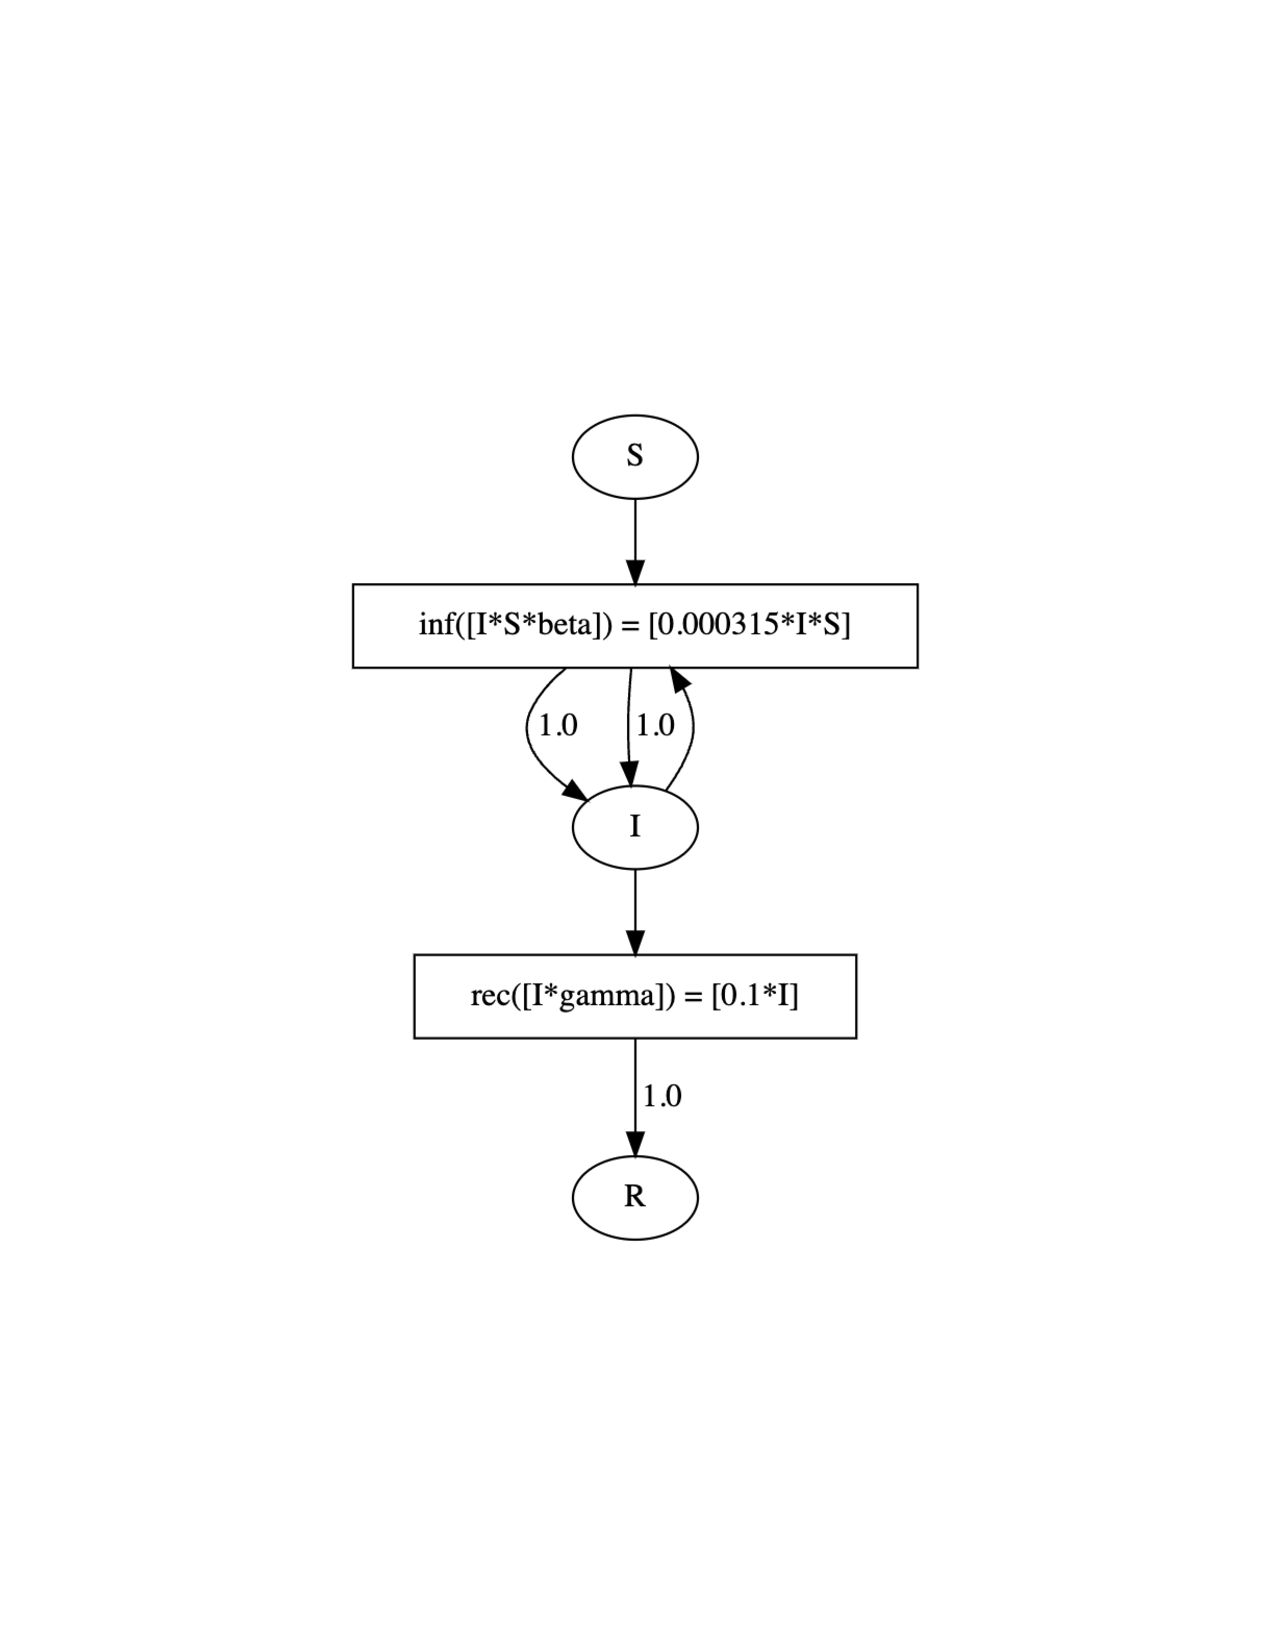
\includegraphics[width=0.3\linewidth,clip]{fig/sir/sir_model.pdf}
    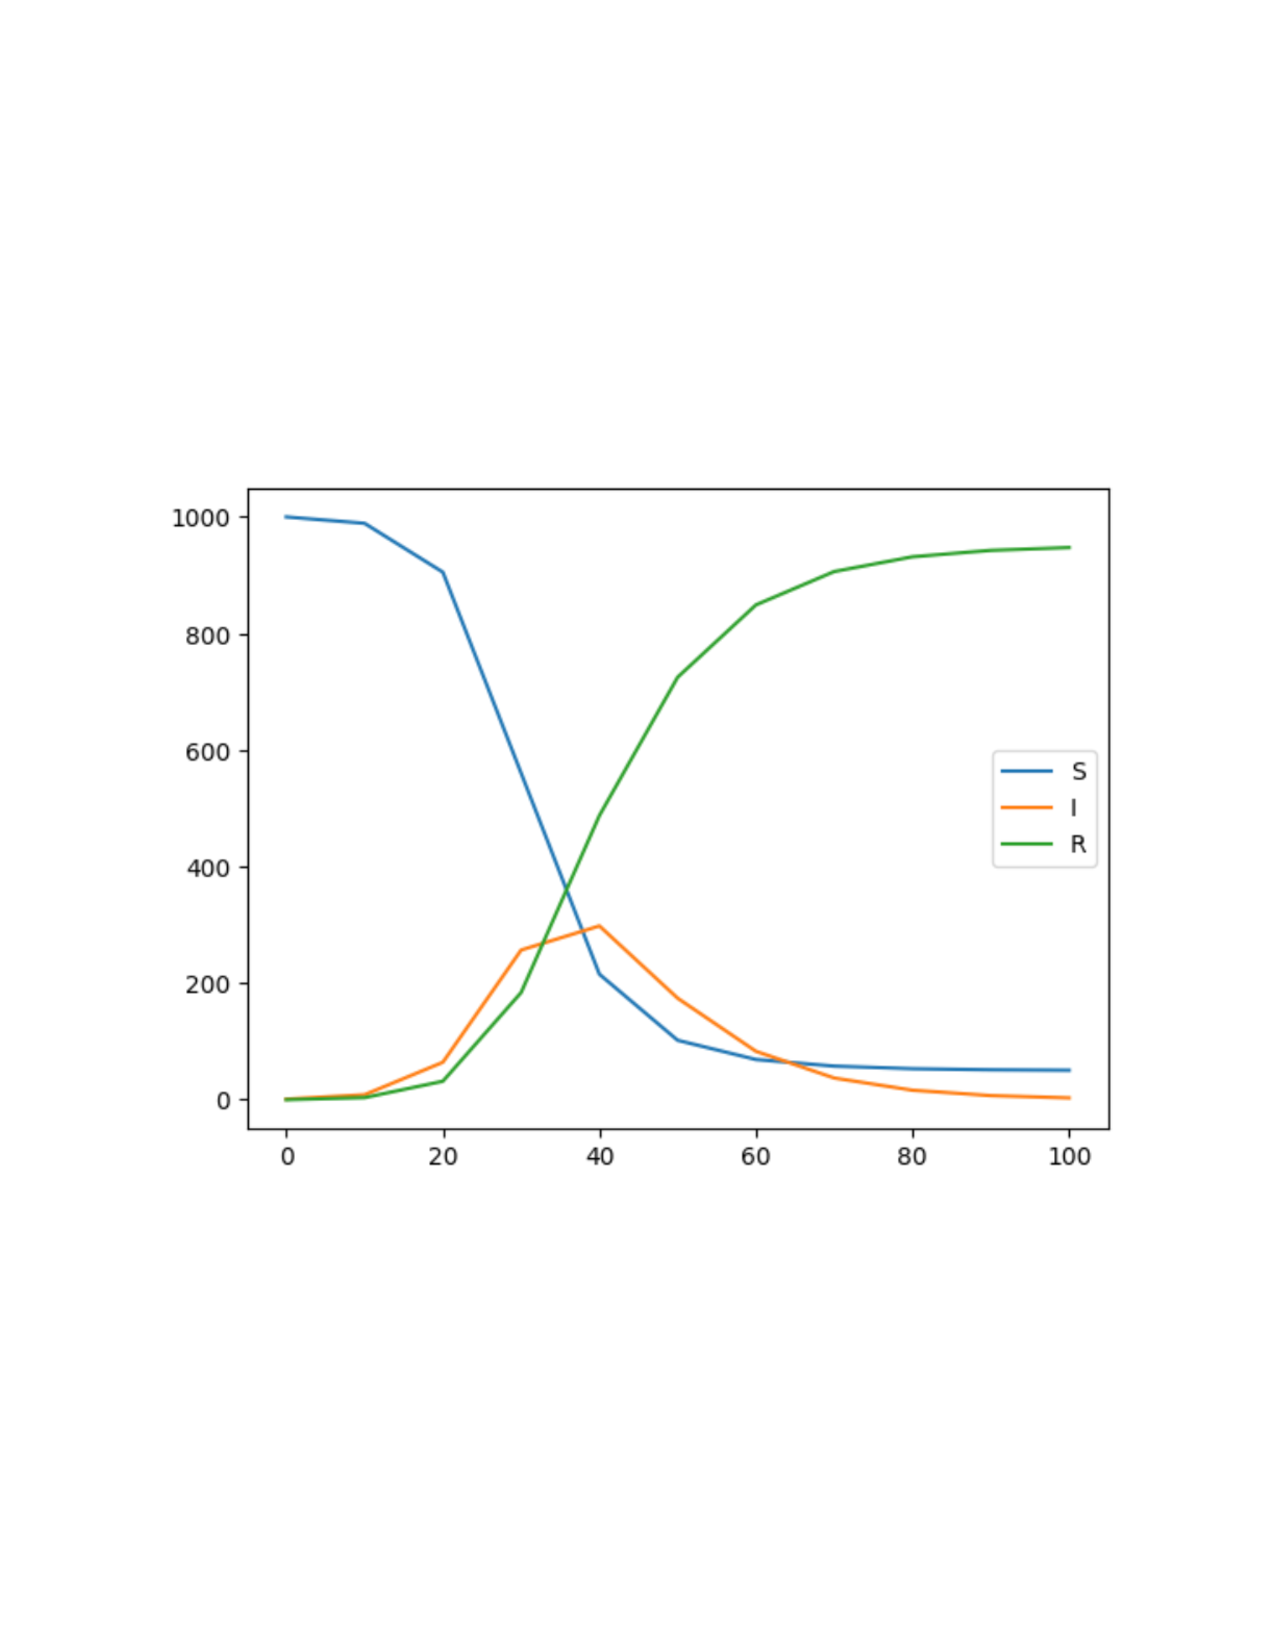
\includegraphics[width=0.4\linewidth,clip]{fig/sir/sir_sim.pdf}

    \caption{\label{fig:sir} Stratified SIR Model (left) and Simulation (right)}
\end{figure}

Figure \ref{fig:sir_bounded} illustrates the baseline SIR after transforming it to bound $S$, $I$, and $R$.  The corresponding lower and upper bounds for each state variable are denoted by a $\_lb$ or $\_ub$ suffix.  The model is different from the baseline in the following ways: there are six state variables and eight transitions, and the transitions use custom rates.  Each baseline transition is replaced by four transitions.  The four transitions differ in whether they define a lower or upper bound, and whether they define the flow into or out from a transition.  For example, the first transition `inf\_in\_lb' defines the lower bound on the flow from $S\_lb$ into the `inf' transition.  The least flow expression is illustrated in the box for the transition.  Simulating this model with the same initial state and parameters (where the lower and upper bounds are initially equal) results in a simulation where the lower and upper bounds are equal for all variables.  While bounding this model in this fashion is not useful in itself, it illustrates a simple application of the bounding transformation.  The bounded abstraction, described below, is similar except that it uses alternative bounds on the parameters.  

\begin{figure}[t]
    \centering
    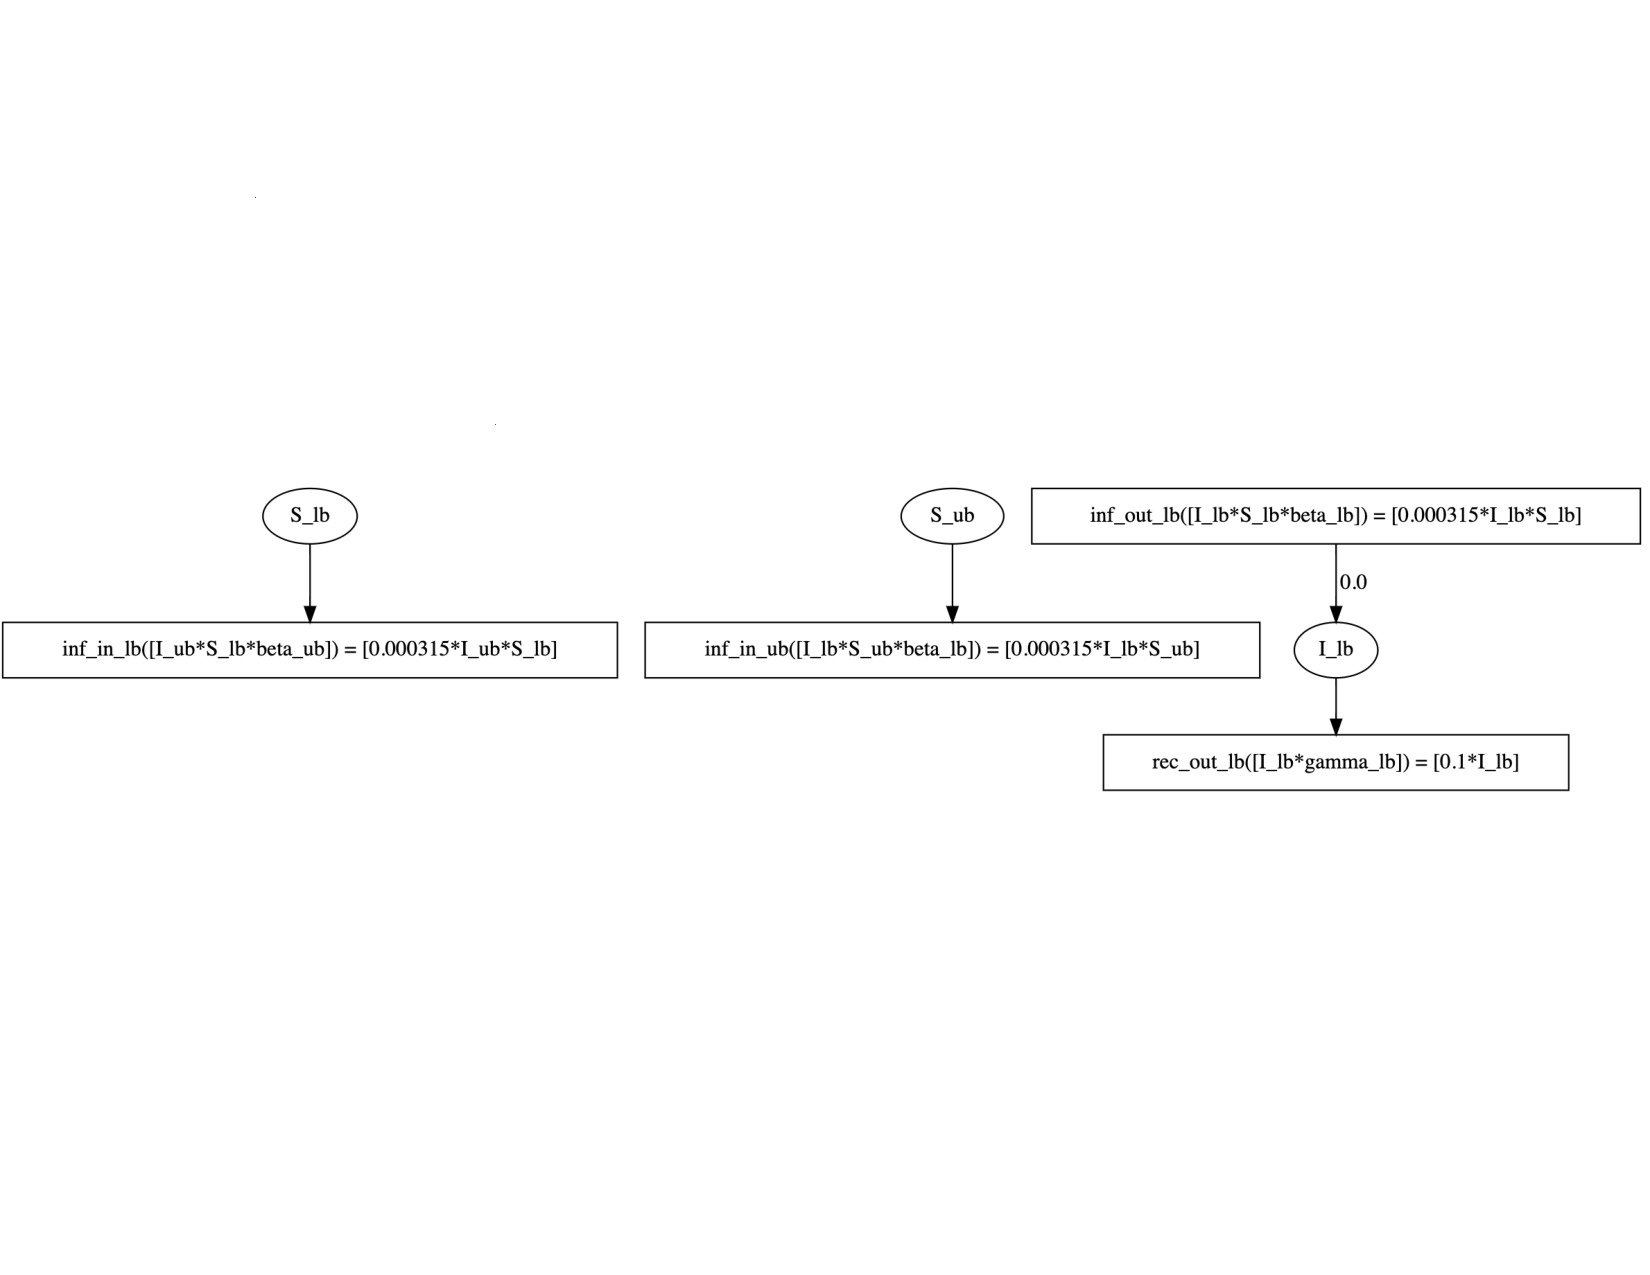
\includegraphics[width=0.8\linewidth,clip,trim={0 8cm 0 8cm}]{fig/sir/sir_bounded_model_1.pdf}
    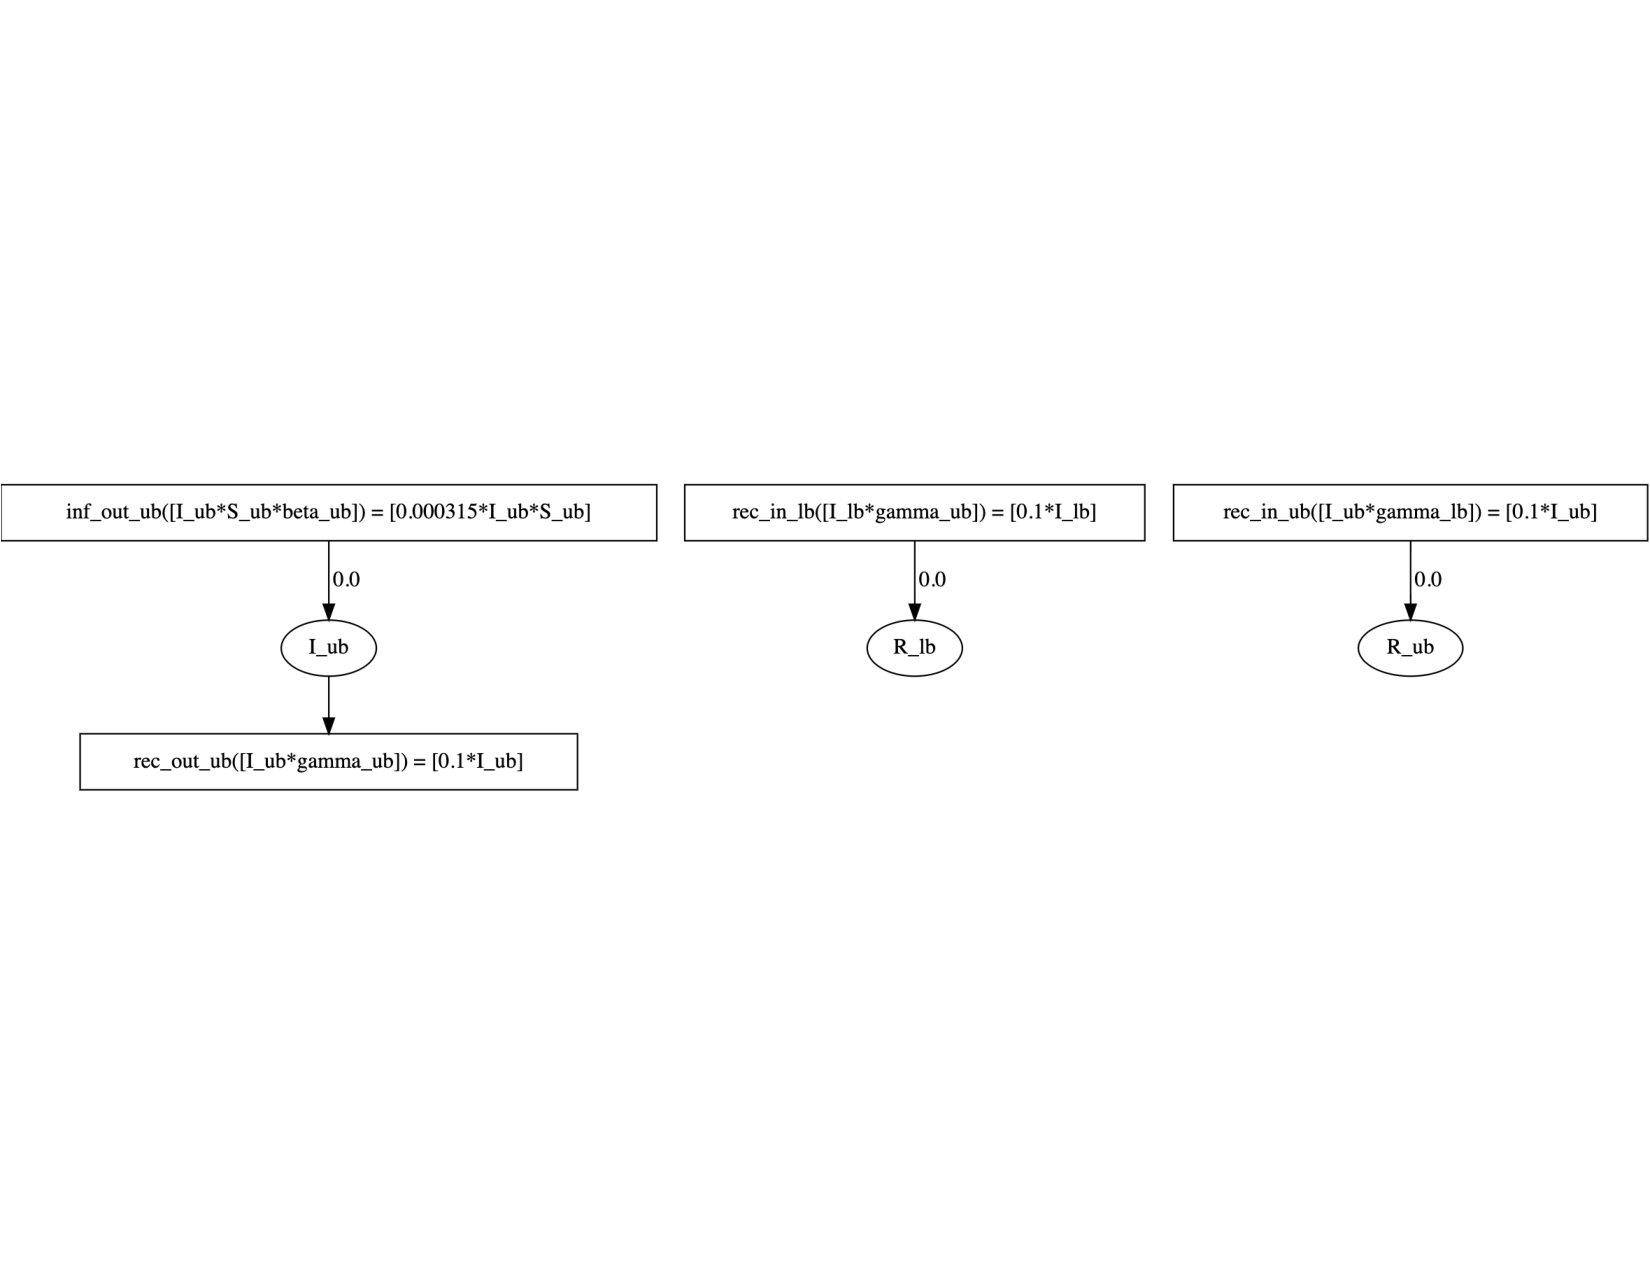
\includegraphics[width=0.8\linewidth,clip]{fig/sir/sir_bounded_model_2.pdf}
    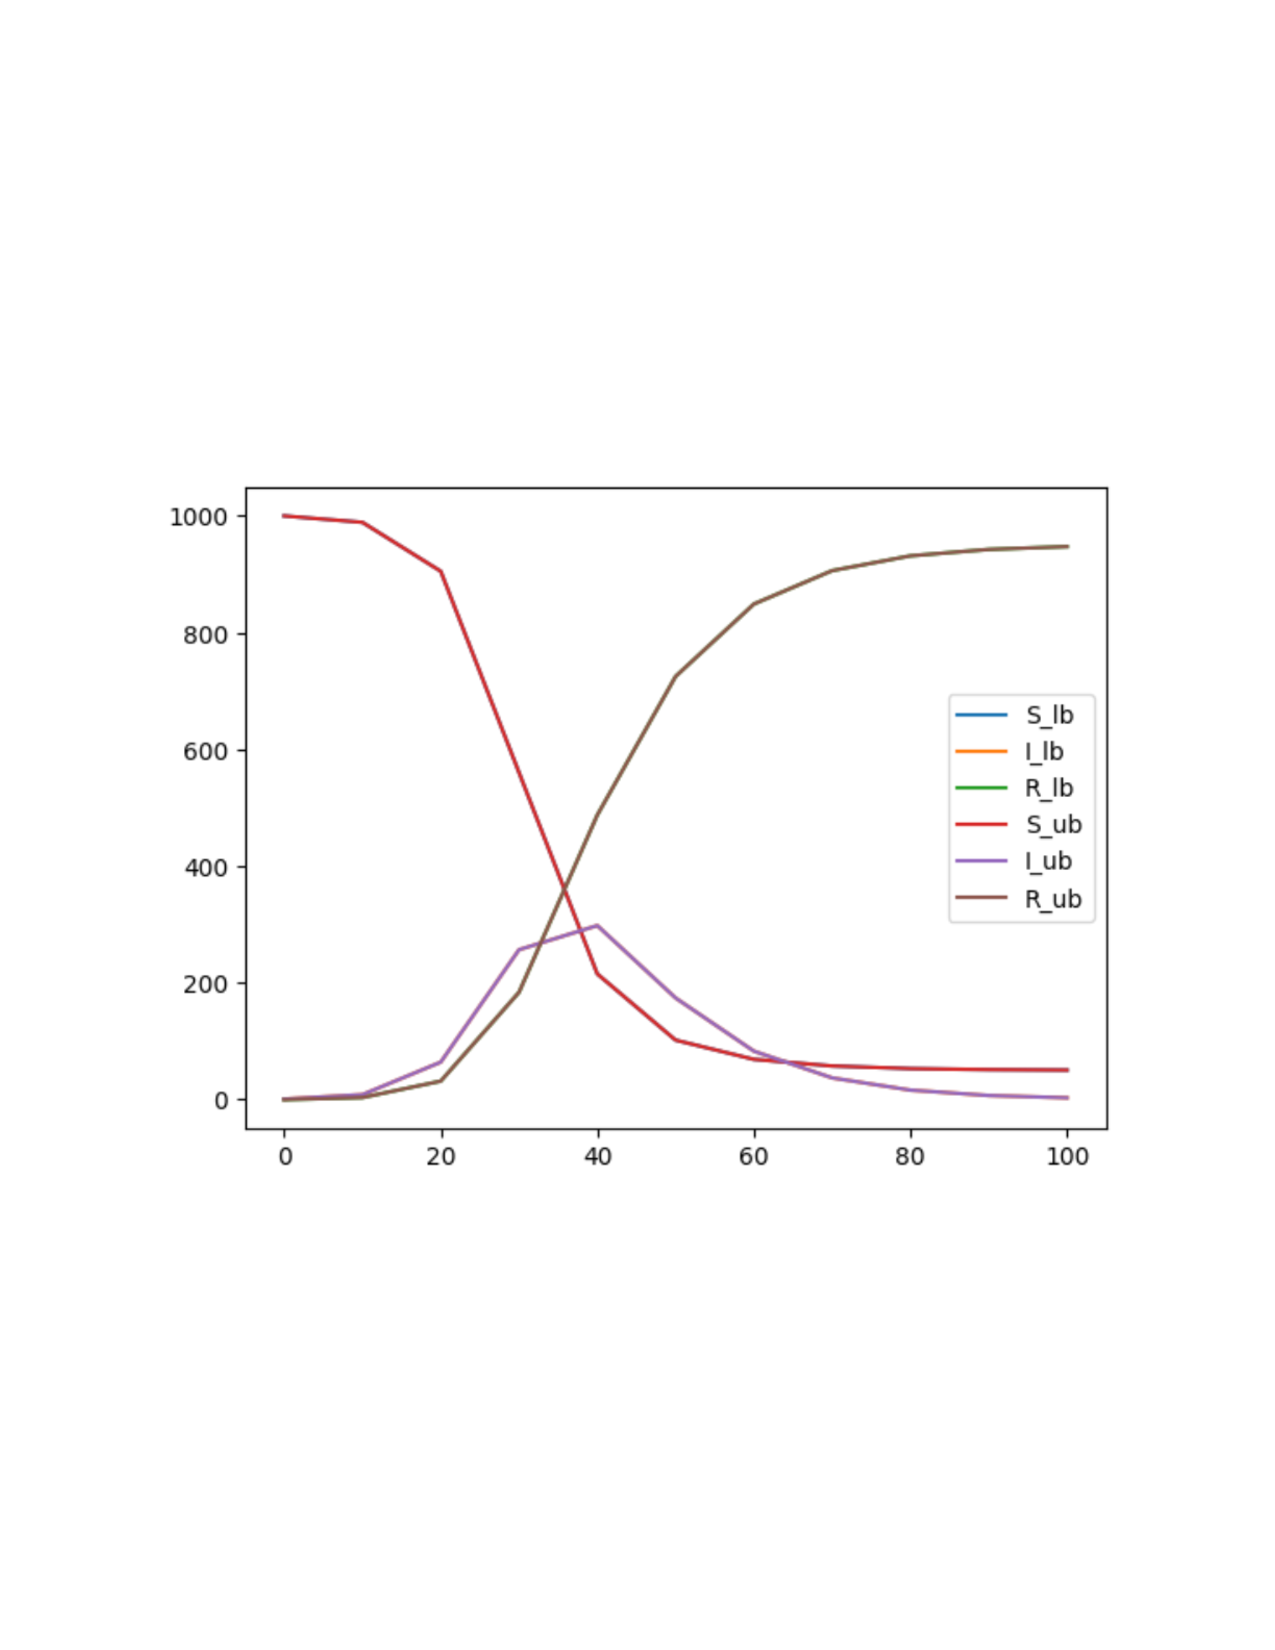
\includegraphics[width=0.4\textwidth,clip]{fig/sir/sir_bounded_sim.pdf}
    \caption{\label{fig:sir_bounded} Bounded SIR Model (top) and Simulation (bottom)}
\end{figure}

Figure \ref{fig:sir_stratified} illustrates the stratified SIR model (wrt. $S$).  It uses state variables that distinguish two $S$ populations and two $inf$ transitions that distinguish different rates due to two $\beta$ parameters.  We modified the $\beta$ parameters to be slightly less and greater than $\beta$ from the previous models.  The simulation illustrates a difference between the $S$ variables.

\begin{figure}[t]
    \centering
    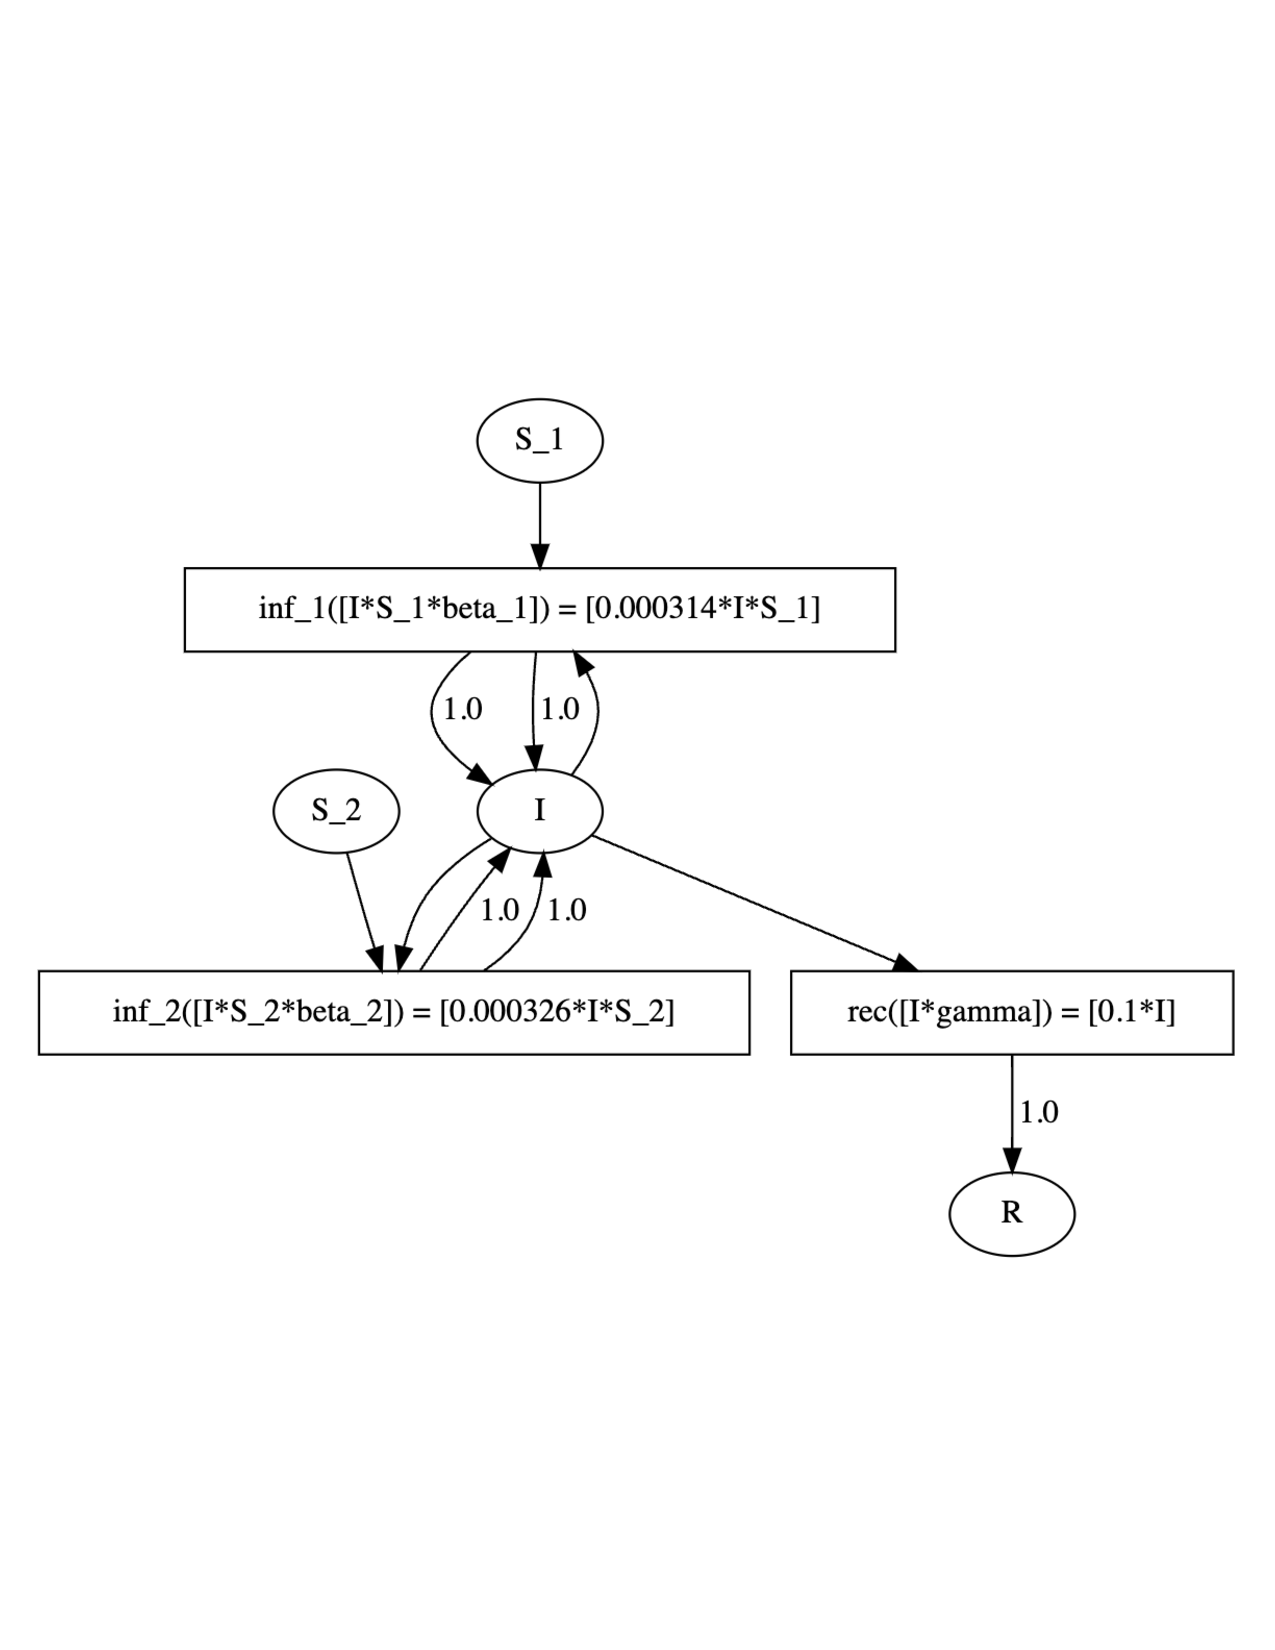
\includegraphics[width=0.5\linewidth,clip]{fig/sir/sir_stratified_model.pdf}
    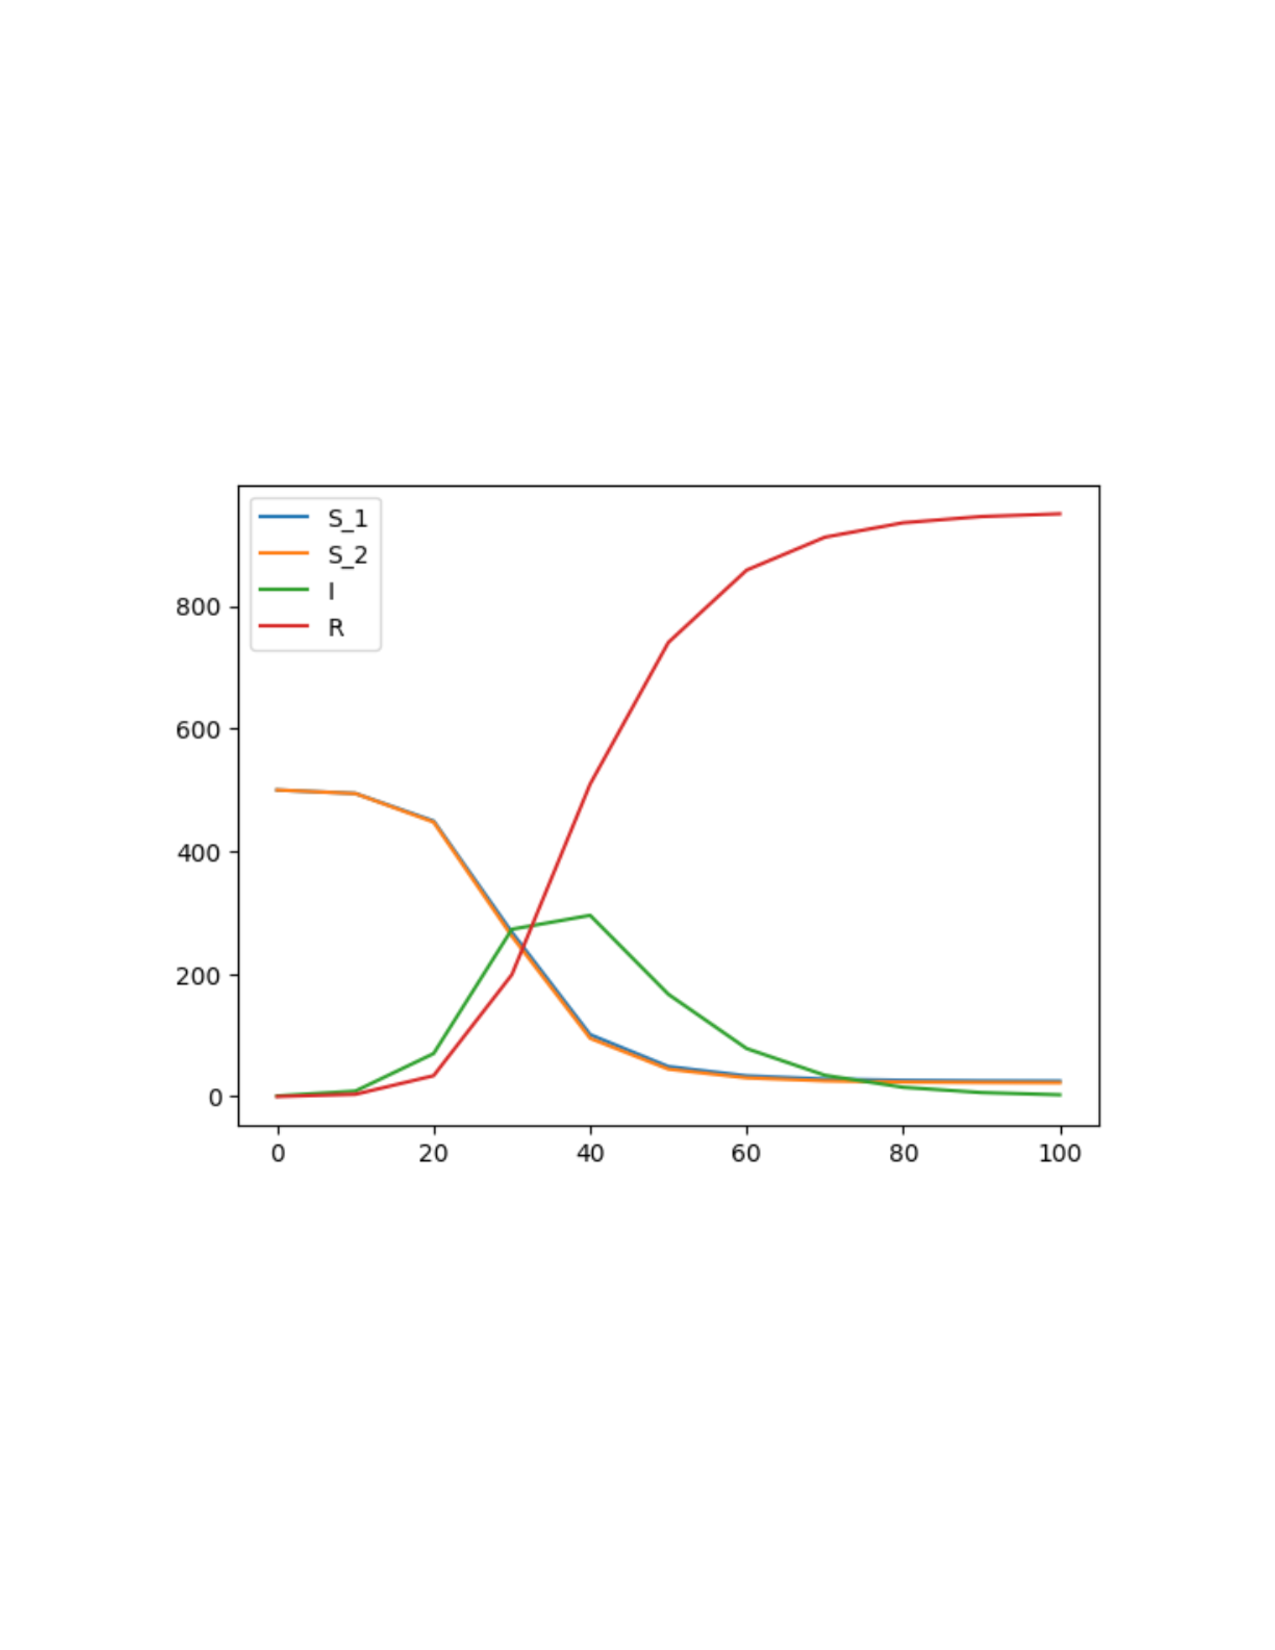
\includegraphics[width=0.4\linewidth,clip]{fig/sir/sir_stratified_sim.pdf}
    \caption{\label{fig:sir_stratified} Stratified SIR Model (top) and Simulation (bottom)}
\end{figure}

Figure \ref{fig:sir_bounded_stratified} illustrates a bounded stratified model, for the sake of illustration.  It resembles the bounded baseline model aside from incorporating the stratified $S$ variable.  The simulation shows how it is possible to bound the stratified variables and achieve similar results to prior models. The primary distinction with this model is how it bounds the stratified variables individually instead of collectively.  The collective bounding can be achieved by first abstracting and then bounding the stratified variables.

\begin{figure}[t]
    \centering
    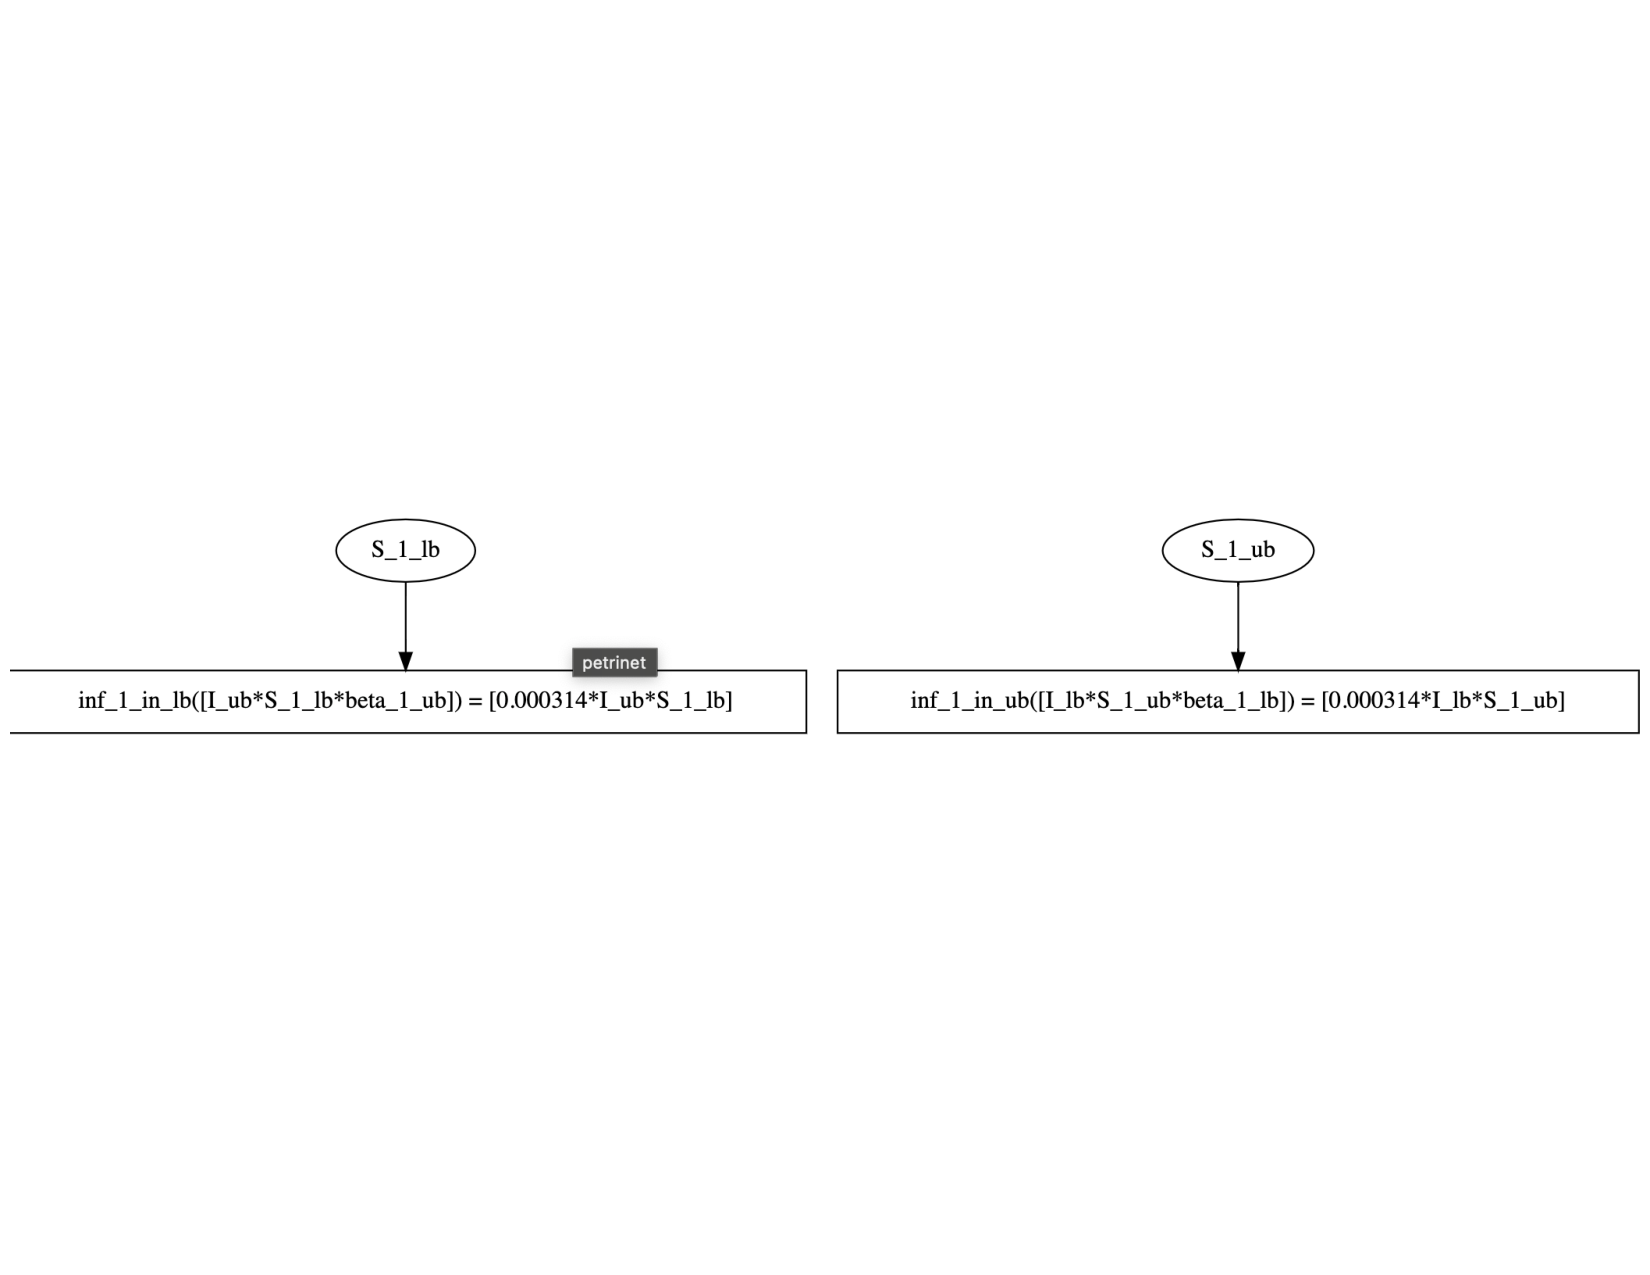
\includegraphics[width=0.6\linewidth,clip]{fig/sir/sir_bounded_stratified_1.pdf}
    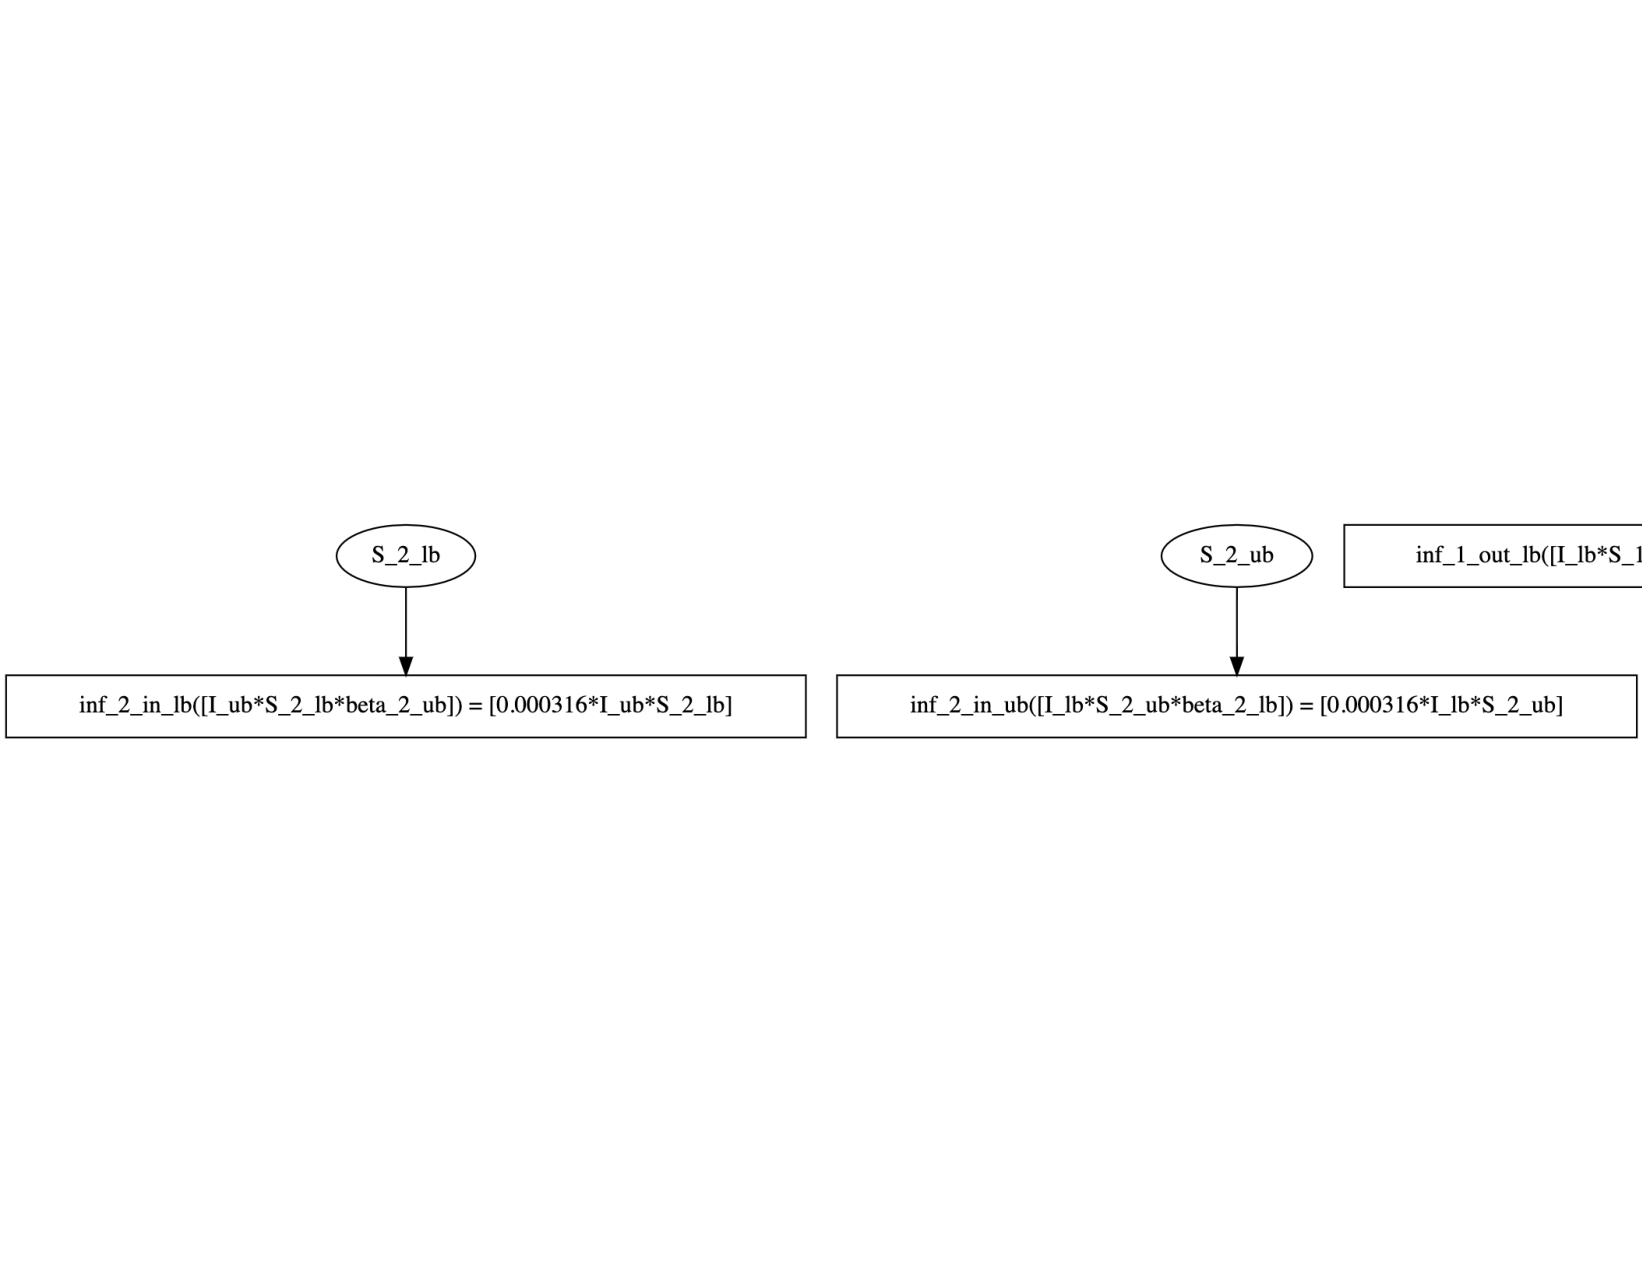
\includegraphics[width=0.6\linewidth,clip]{fig/sir/sir_bounded_stratified_2.pdf}
    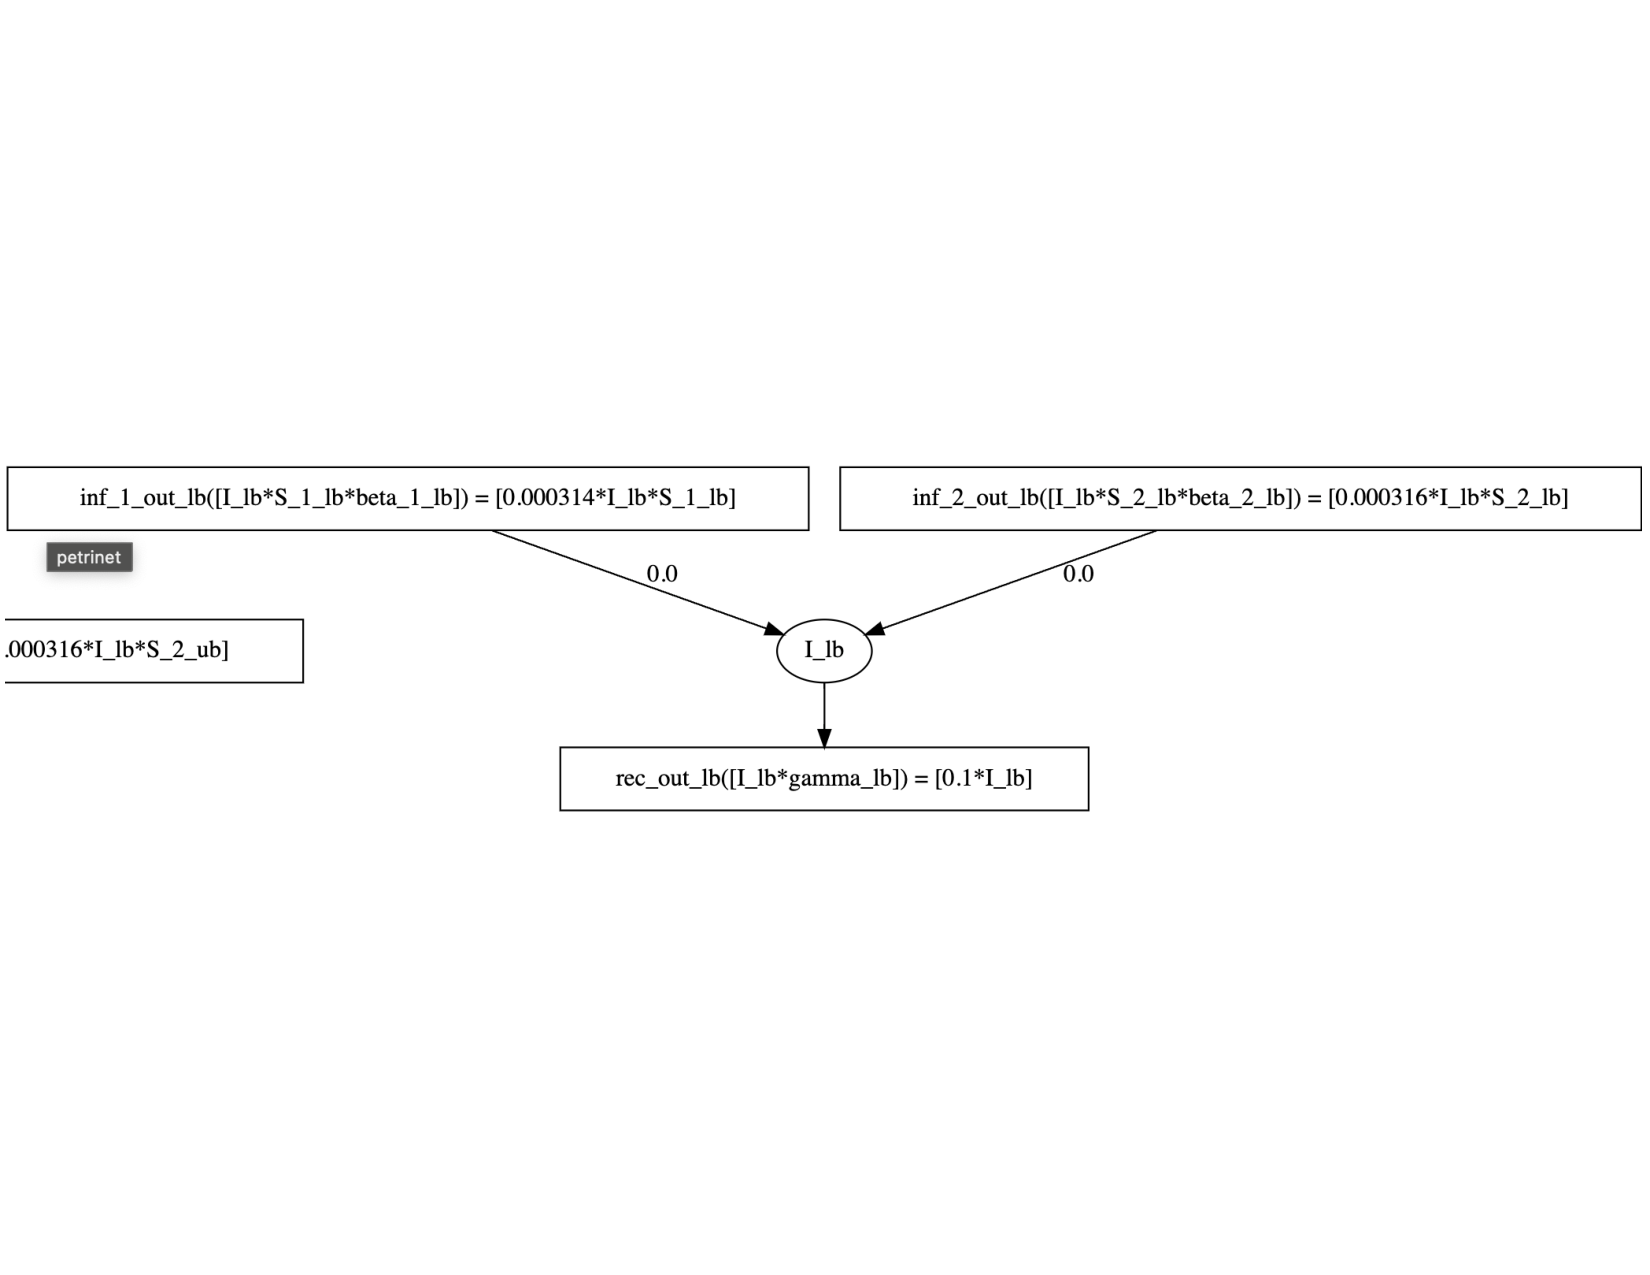
\includegraphics[width=0.6\linewidth,clip]{fig/sir/sir_bounded_stratified_3.pdf}
    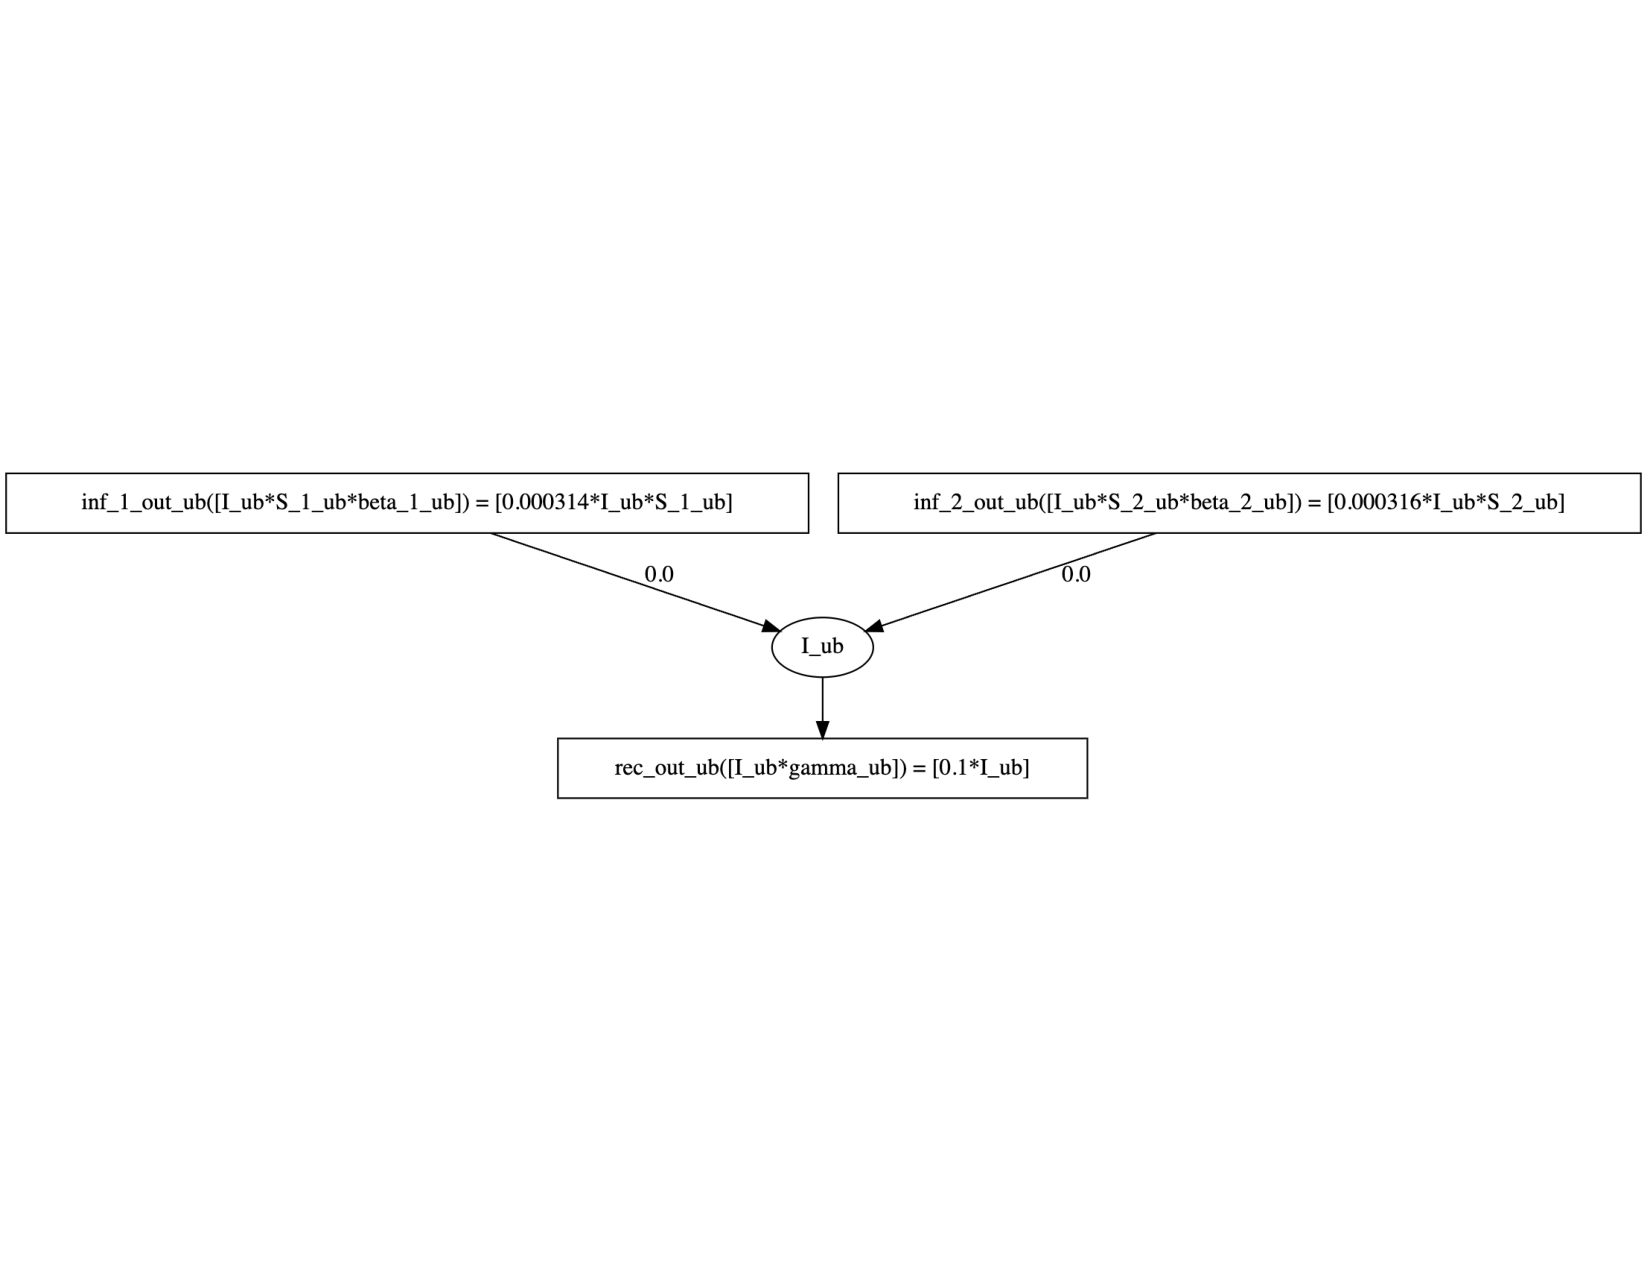
\includegraphics[width=0.6\linewidth,clip]{fig/sir/sir_bounded_stratified_4.pdf}
    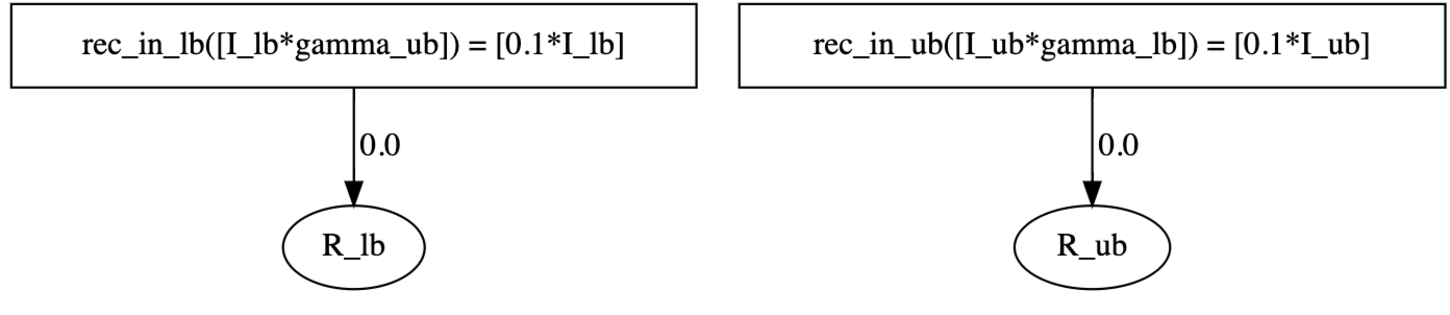
\includegraphics[width=0.4\linewidth,clip]{fig/sir/sir_bounded_stratified_5.pdf}\\
    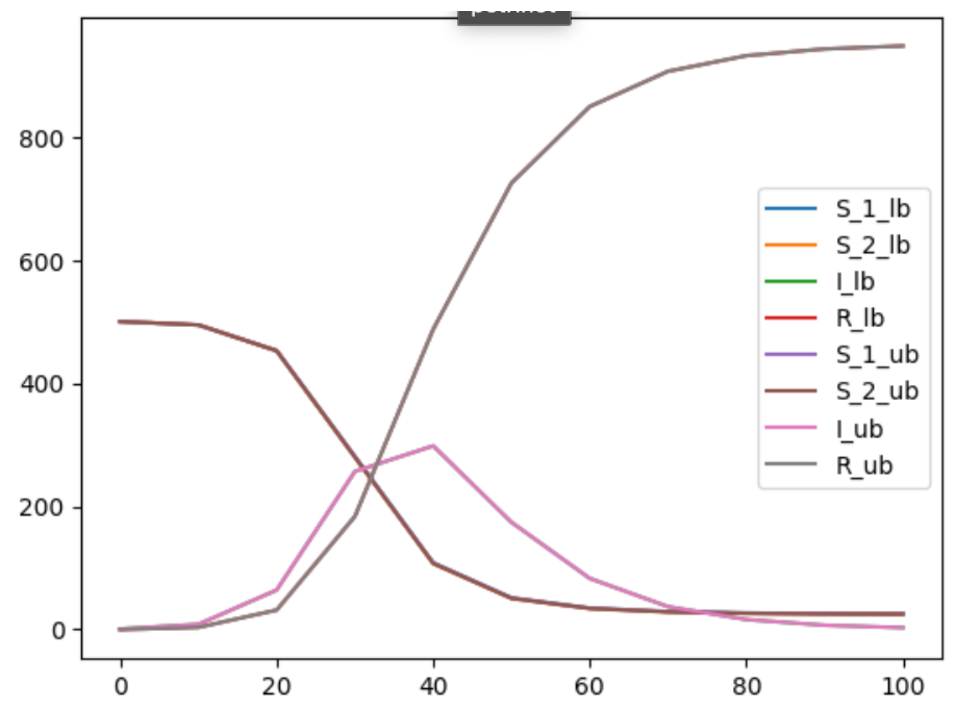
\includegraphics[width=0.4\linewidth,clip]{fig/sir/sir_bounded_stratified_sim.pdf}
    \caption{\label{fig:sir_bounded_stratified} Bounded Stratified SIR Model (top) and Simulation (bottom)}
\end{figure}


Figure \ref{fig:sir_abstract_bounded_stratified}  illustrates the bounded abstracted model.  It resembles the bounded baseline model, except that it incorporates upper and lower bounds on the $\beta$ parameter due to the stratified populations.  By propagating lower and upper bounds that are not equal, this variation of the model captures lower and upper bounds on the abstracted state variables.  The bounds are tight enough to answer several queries about the model.  For example, it can assess whether a upper threshold (that does not fall between the bounds) on peak infected $I$ is satisfied.  The threshold $I \leq 400$ is satisfied because $I\_ub \leq 400$.  However, the threshold $I \leq 300$ may or may not be satisfied because $I\_lb \leq 300 \leq I\_ub$.

\begin{figure}[t]
    \centering
    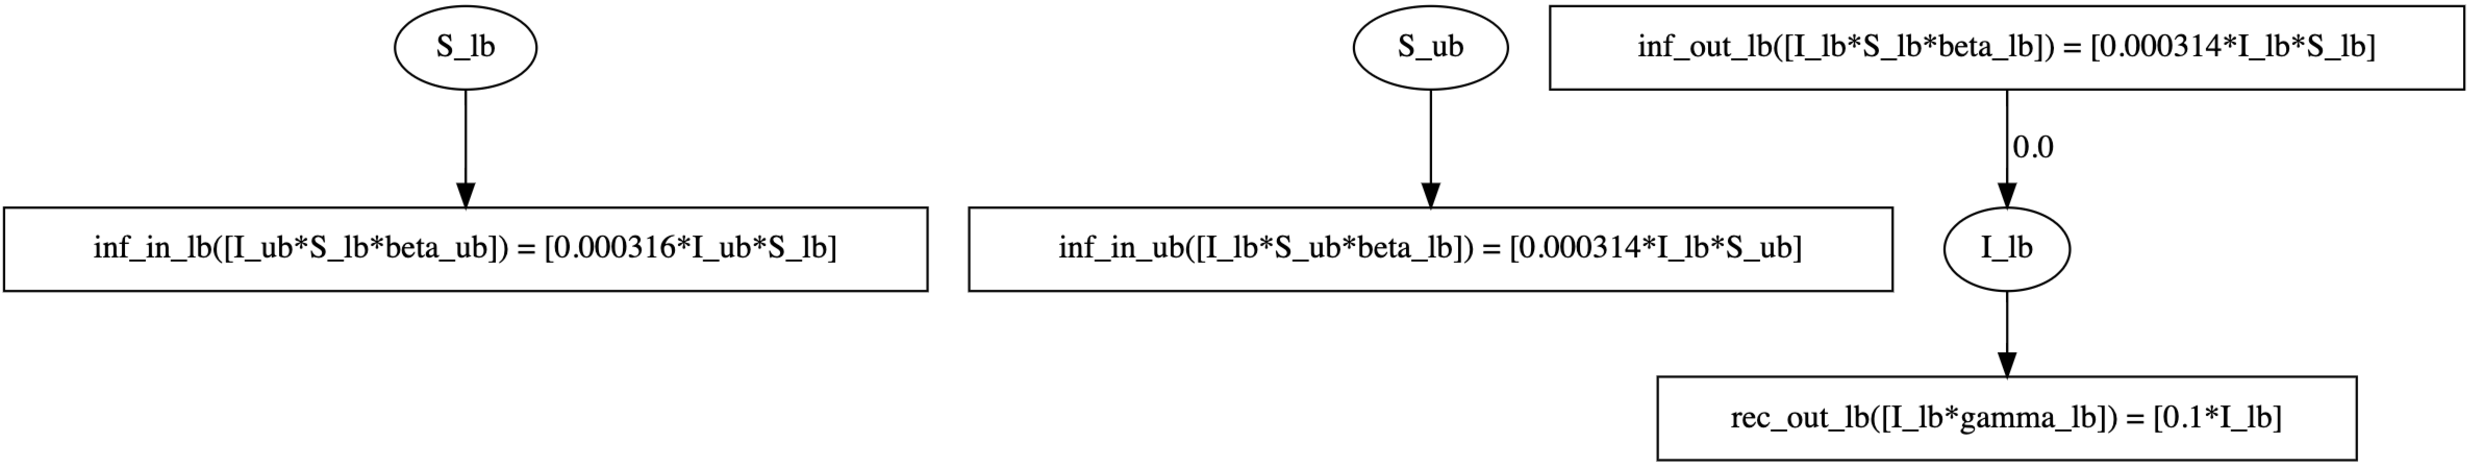
\includegraphics[width=0.6\linewidth,clip]{fig/sir/sir_abstract_bounded_model_1.pdf}
    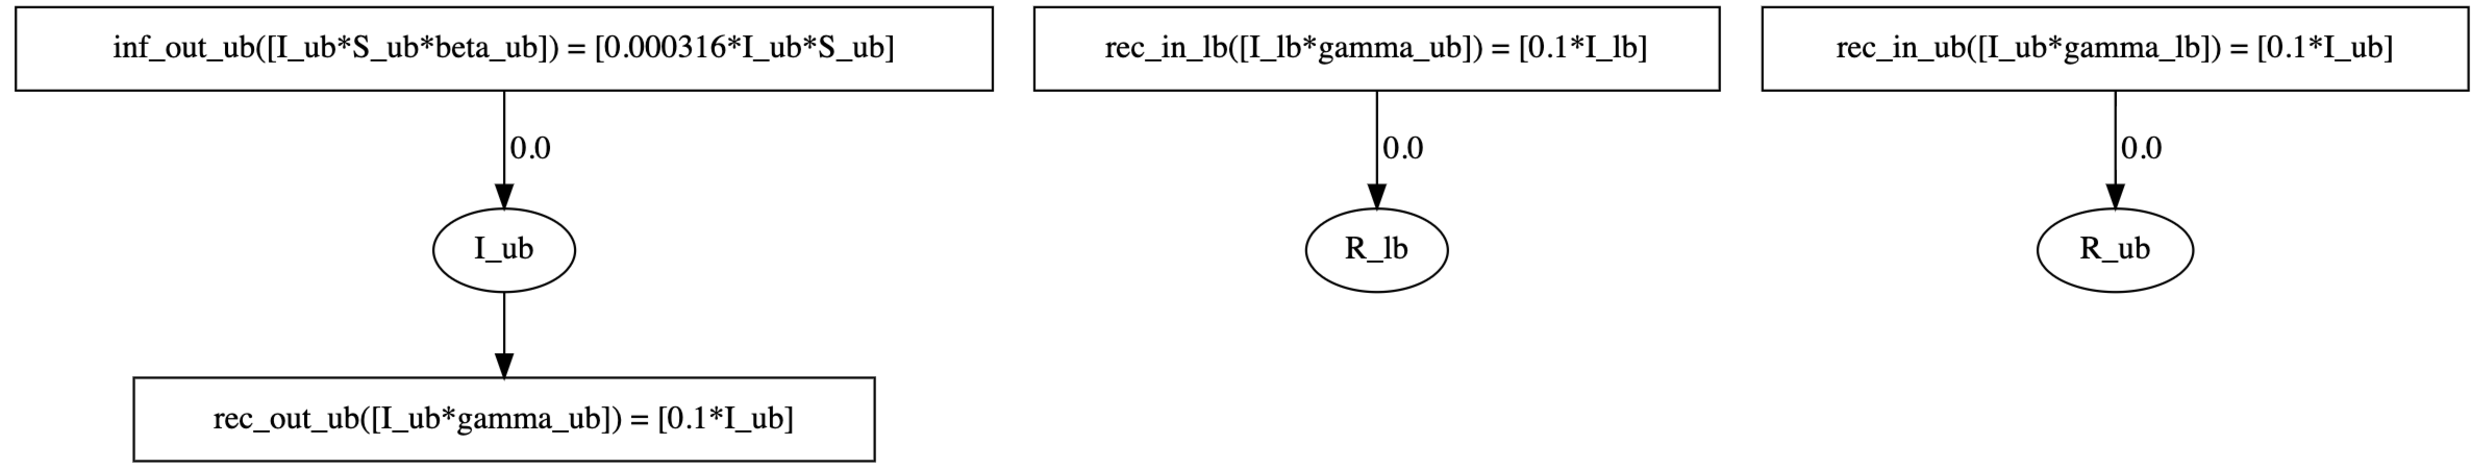
\includegraphics[width=0.6\linewidth,clip]{fig/sir/sir_abstract_bounded_model_2.pdf}
    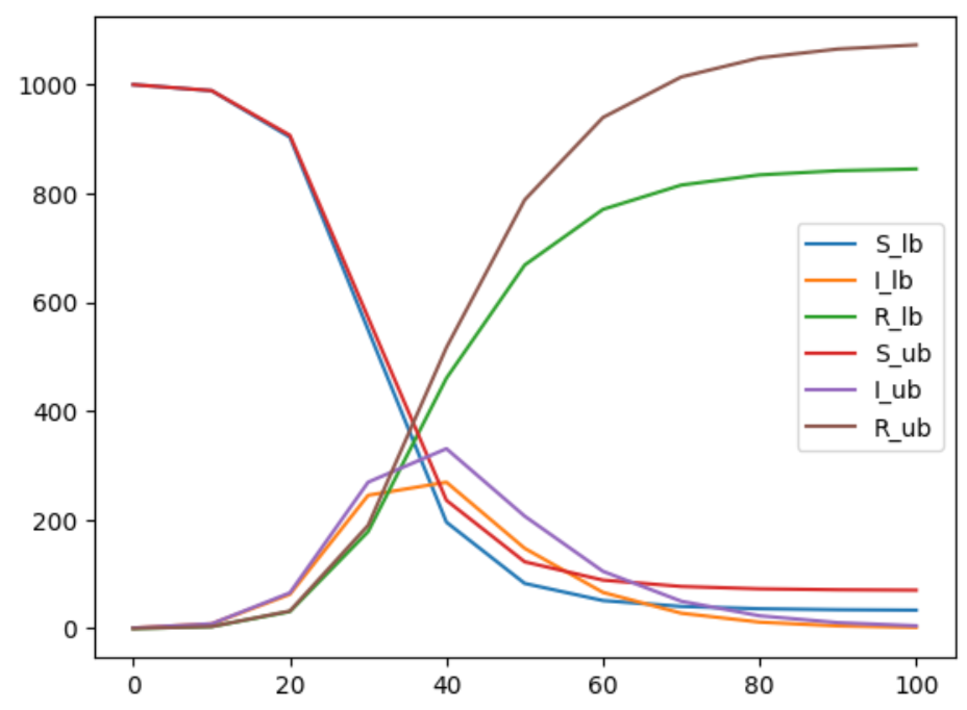
\includegraphics[width=0.4\linewidth,clip]{fig/sir/sir_abstract_bounded_sim.pdf}
    \caption{\label{fig:sir_abstract_bounded_stratified} Bounded Stratified SIR Model (top) and Simulation (bottom)}
\end{figure}

% \begin{figure}
%     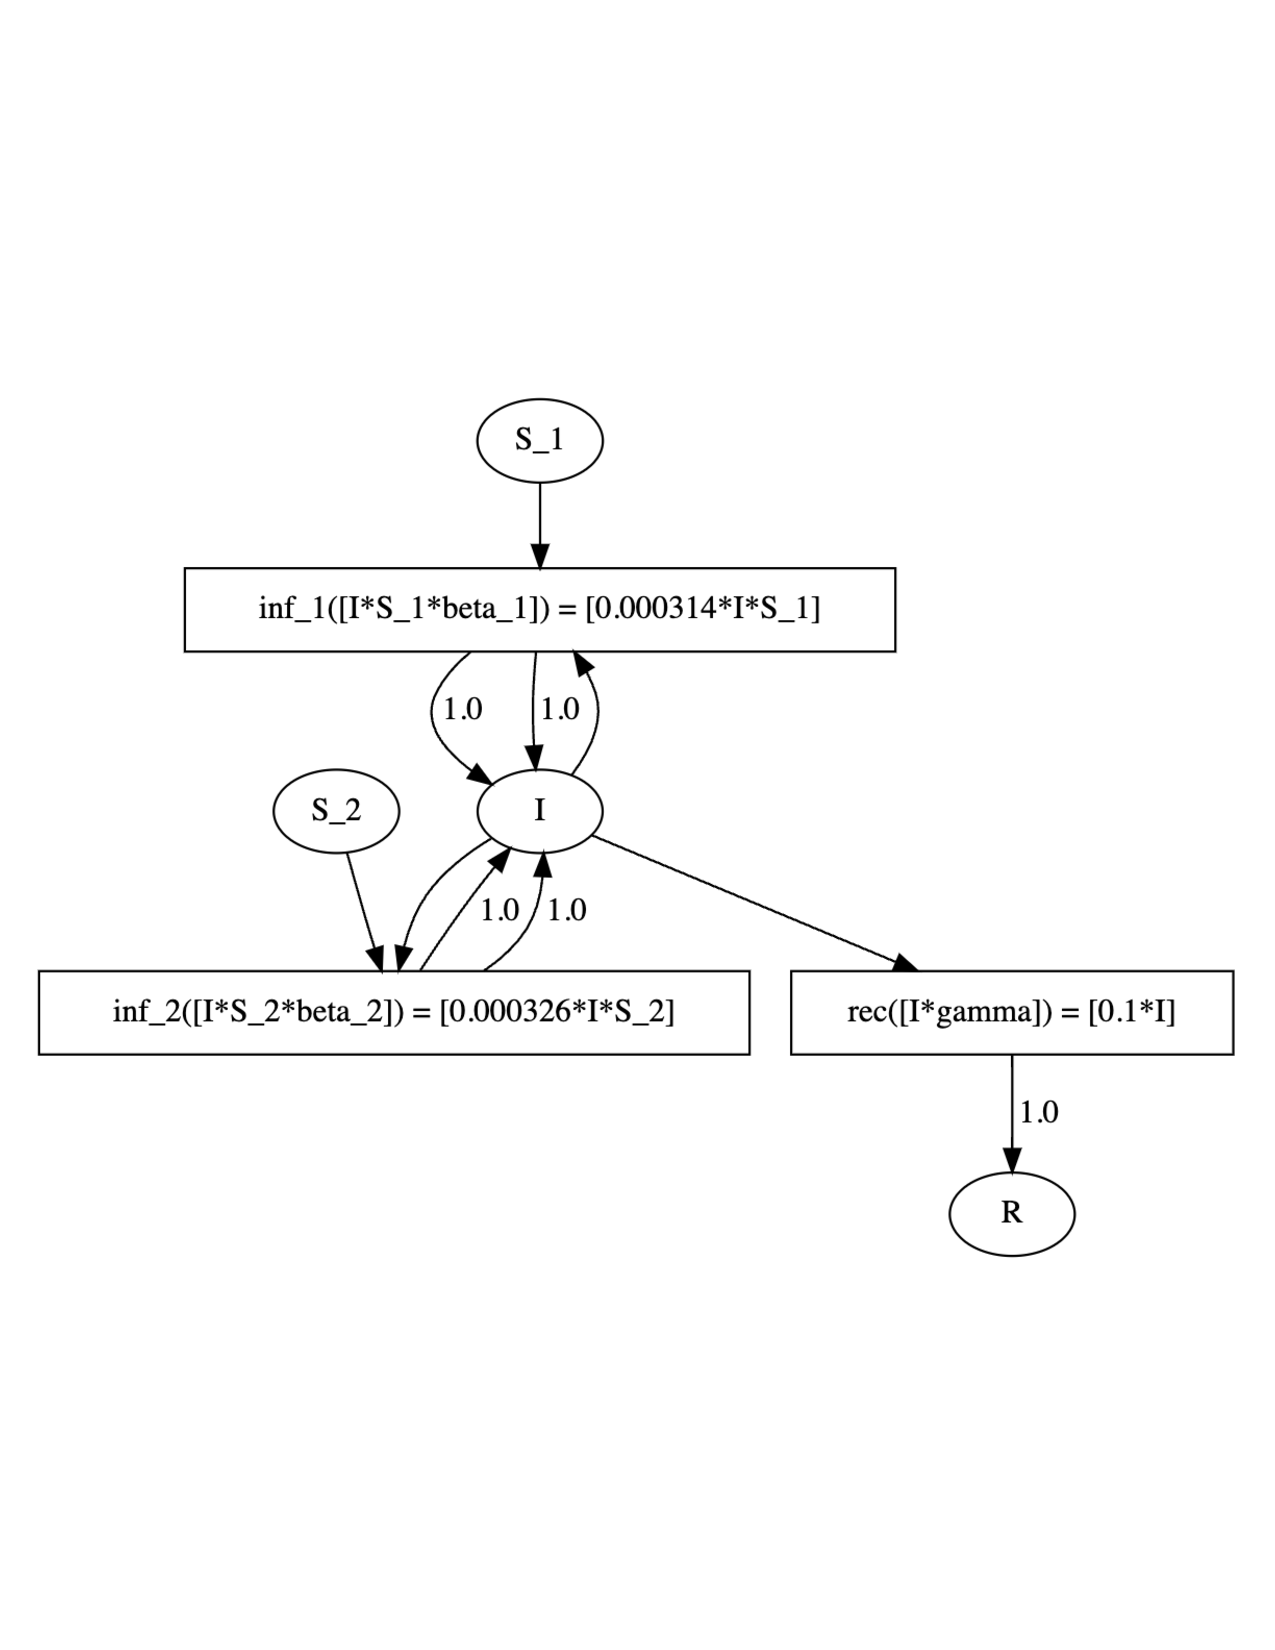
\includegraphics[width=\linewidth]{fig/sir/sir_stratified_model.pdf}
% %     \caption{\label{fig:sir_stratified_model} Stratified SIR Model}
% % \end{figure}

% % \begin{figure}
%     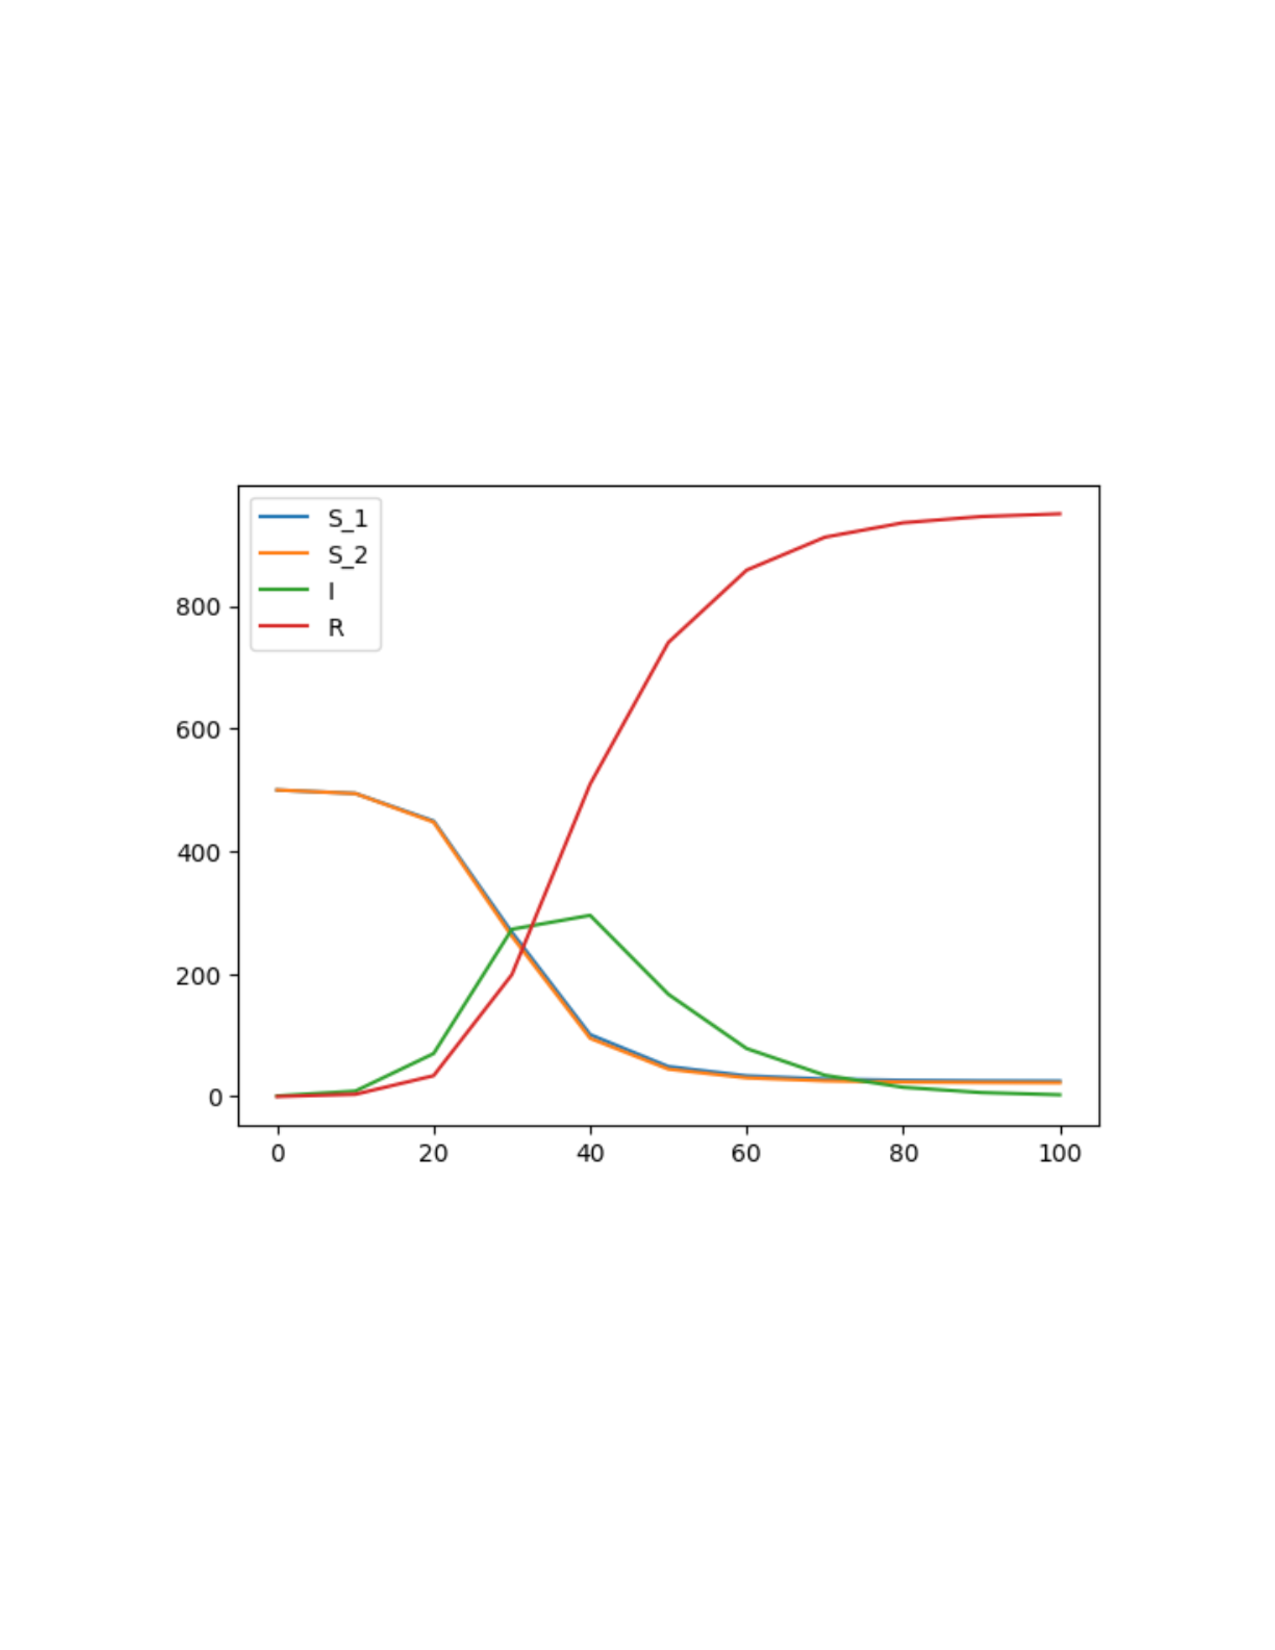
\includegraphics[width=\linewidth]{fig/sir/sir_stratified_sim.pdf}
%     \caption{\label{fig:sir_stratified_sim} Stratified SIR Model (top) and Simulation (bottom)}
% \end{figure}

% \section{Stratification Abstraction}
% The SIERHD model from the July monthly demo uses the model summarized by the Petrinet diagram in Figure \ref{fig:seirhd}.

\begin{figure}
    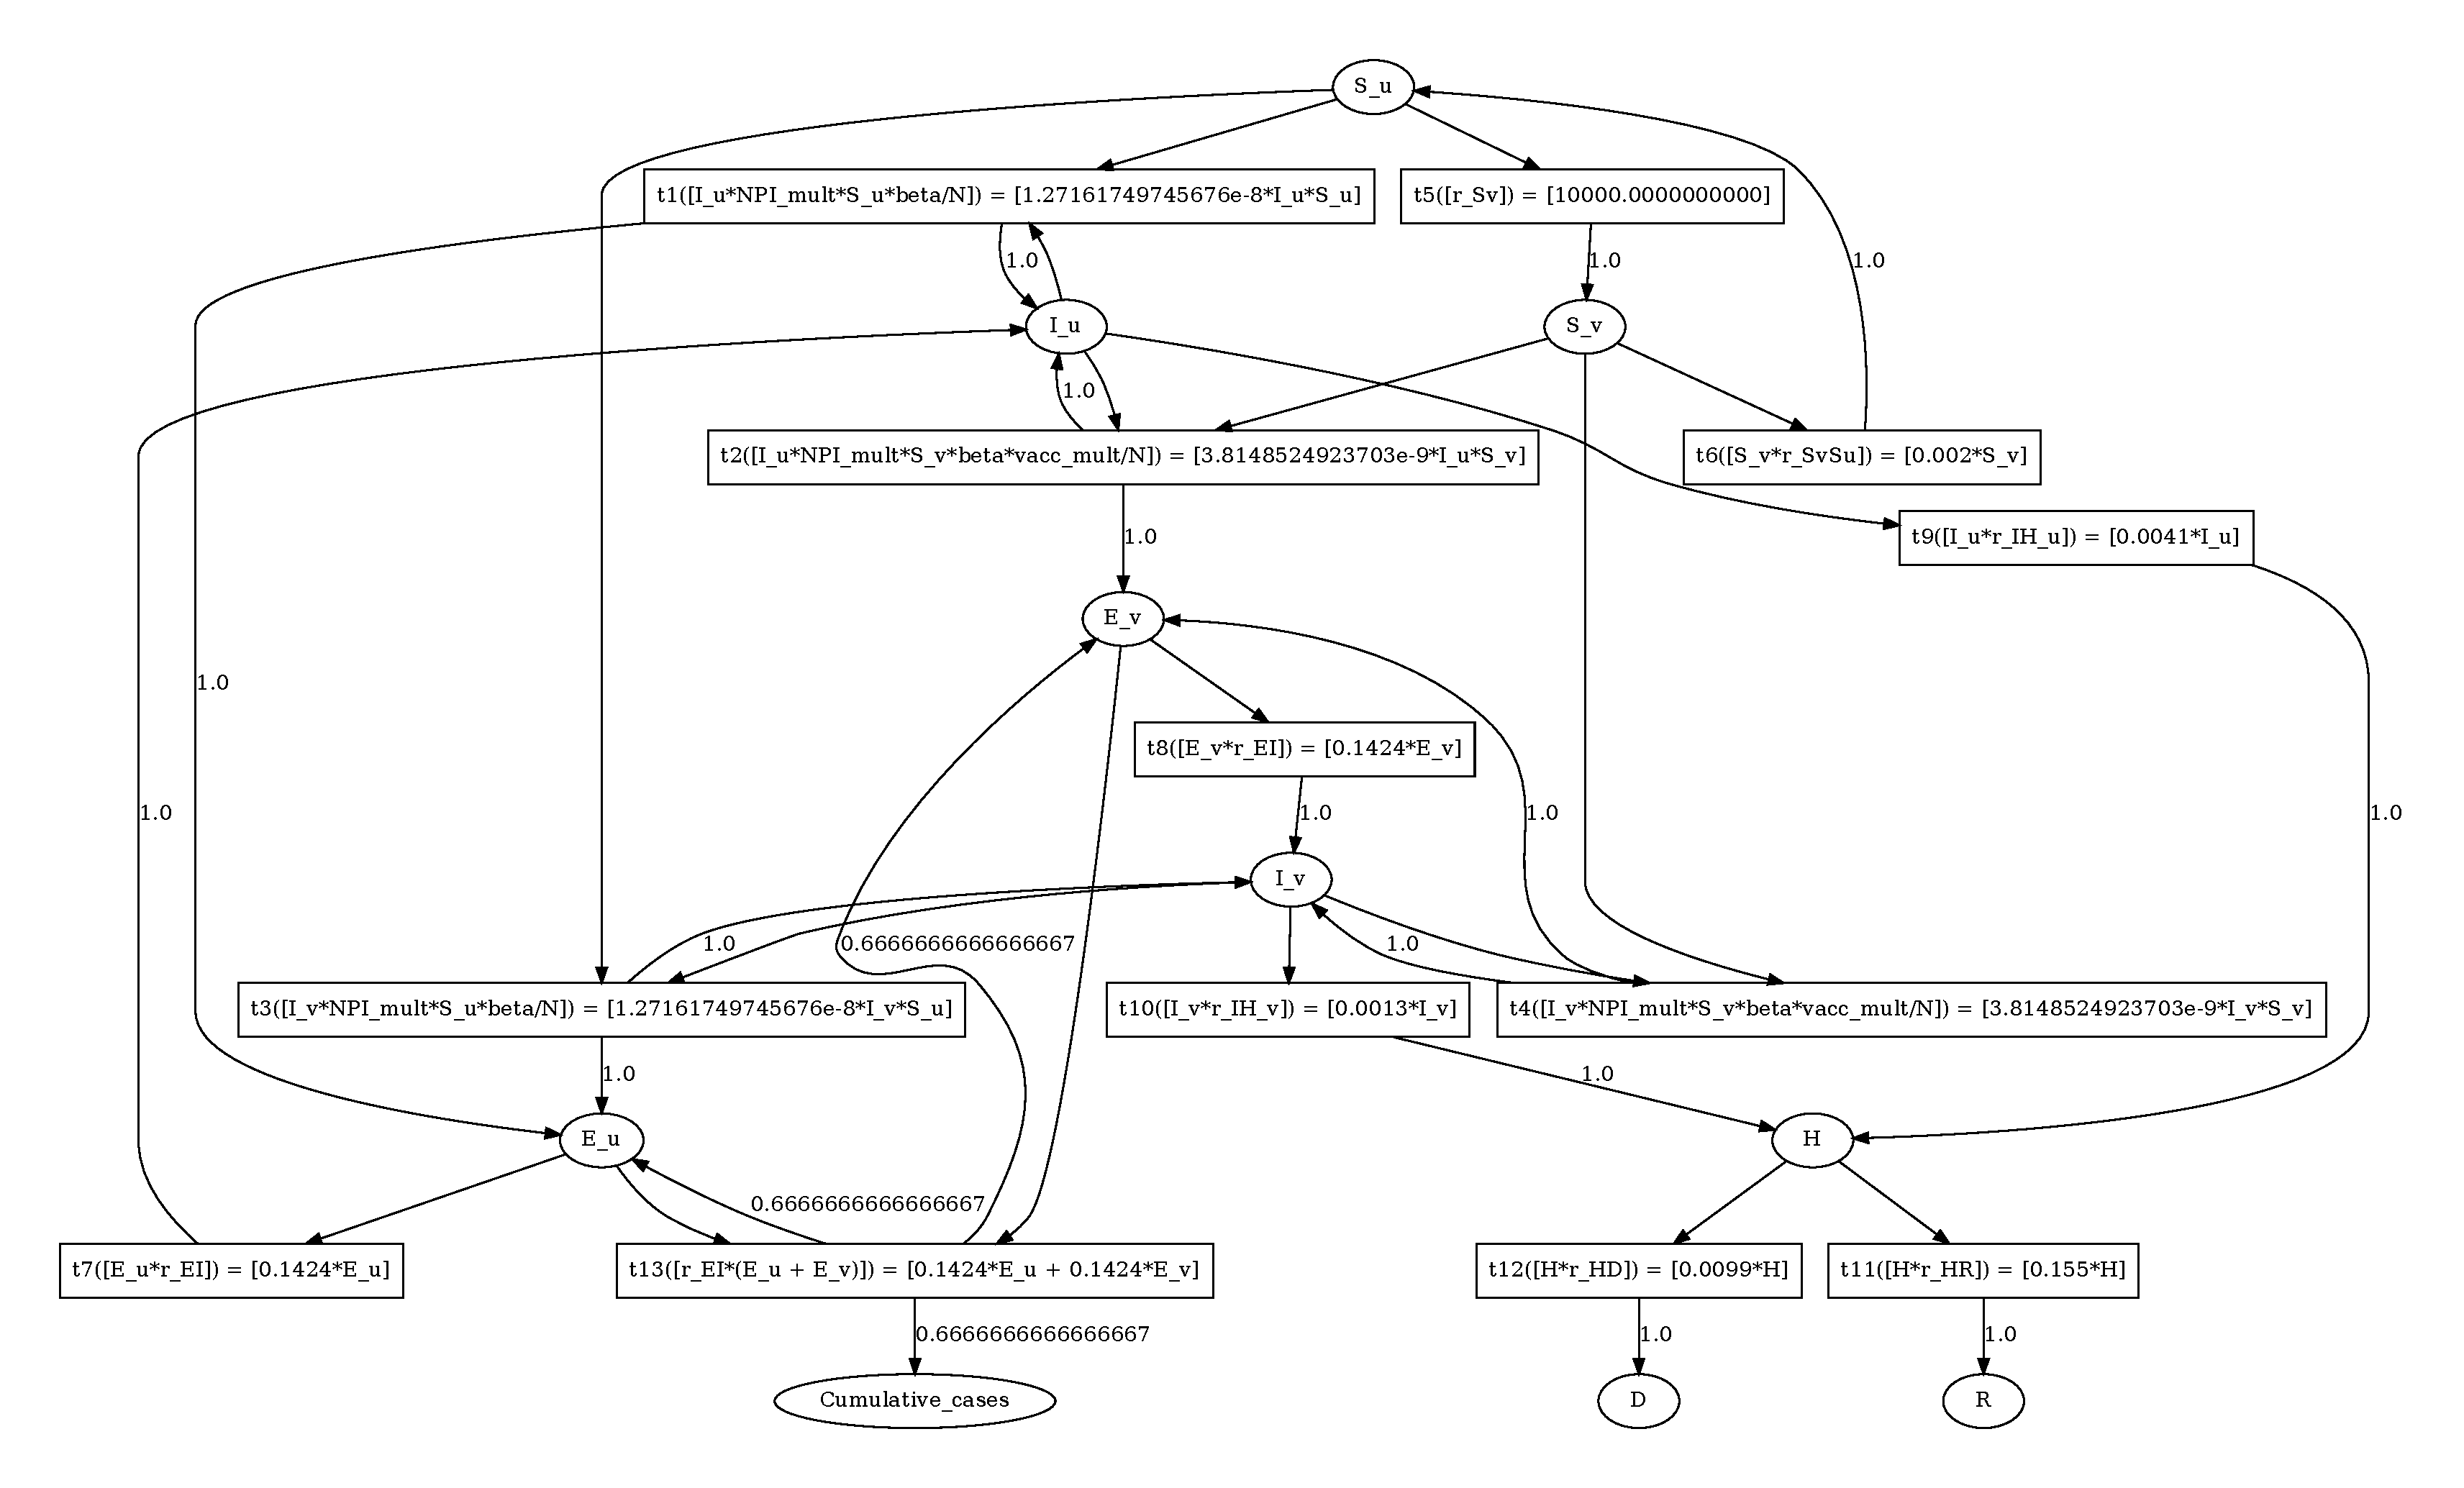
\includegraphics[width=\linewidth]{fig/seirhd}
    \caption{\label{fig:seirhd} SEIRHD Model Petrinet}
\end{figure}

The following transitions connect the variables $S_u$, $S_v$, $E_u$, $E_v$, $I_u$, and $I_v$:

\begin{eqnarray*}
    (I_u, S_u) &\xrightarrow[]{r_1}& (I_u, E_u)\\
    (I_u, S_v) &\xrightarrow[]{r_2}& (I_u, E_v)\\
    (I_v, S_u) &\xrightarrow[]{r_3}& (I_v, E_u)\\
    (I_v, S_v) &\xrightarrow[]{r_4}& (I_v, E_v)\\
    (S_u) &\xrightarrow[]{r_5}& (S_v)\\
    (S_v) &\xrightarrow[]{r_6}& (S_u)\\
    (E_u) &\xrightarrow[]{r_7}& (I_u)\\
    (E_v) &\xrightarrow[]{r_8}& (I_v)
\end{eqnarray*}

Recovering the original, unstratified model corresponds to an abstraction where $S = (S_u, S_v)$, $I = (I_u, I_v)$, and $E = (E_u, E_v)$: 

\begin{eqnarray*}
    (I, S) &\xrightarrow[]{r_1}& (I, E)\\
    (I, S) &\xrightarrow[]{r_2}& (I, E)\\
    (I, S) &\xrightarrow[]{r_3}& (I, E)\\
    (I, S) &\xrightarrow[]{r_4}& (I, E)\\
    (S) &\xrightarrow[]{r_5}& (S)\\
    (S) &\xrightarrow[]{r_6}& (S)\\
    (E) &\xrightarrow[]{r_7}& (I)\\
    (E) &\xrightarrow[]{r_8}& (I)
\end{eqnarray*}

In order for the abstraction to preserve the semantics of the stratified model, it must define $S^t = S_u^t + S_v^t$, $I^t = I_u^t + I_v^t$, and $E^t = E_u^t + E_v^t$ for all time points $t$.  If we look at the definitions for these terms, we have:

\begin{eqnarray*}
    \frac{\partial S_u}{\partial t} &=& - I_u S_u r_1 - I_v S_u r_3 - S_u r_5 + S_v r_6\\
    \frac{\partial S_v}{\partial t} &=& - I_u S_v r_2 - I_v S_v r_4 + S_u r_5 - S_v r_6\\ 
    \frac{\partial S}{\partial t} &=& \frac{\partial S_u}{\partial t}  + \frac{\partial S_v}{\partial t} \\
    &=& - I_u S_u r_1 - I_v S_u r_3 - S_u r_5 + S_v r_6 - I_u S_v r_2 - I_v S_v r_4 + S_u r_5 - S_v r_6\\
    &=& - I_u S_u r_1 - I_v S_u r_3 - I_u S_v r_2 - I_v S_v r_4 \\
\end{eqnarray*}

\begin{eqnarray*}
    \frac{\partial I_u}{\partial t} &=& I_u S_u r_1 - I_u S_u r_1 + I_u S_v r_2 - I_u S_v r_2 + E_u r_7\\
    &=&  E_u r_7\\
    \frac{\partial I_v}{\partial t} &=& I_v S_u r_3 - I_v S_u r_3 + I_v S_v r_4 - I_v S_v r_4 + E_v r_8\\ 
    &=& E_v r_8\\ 
    \frac{\partial I}{\partial t} &=& \frac{\partial I_u}{\partial t}  + \frac{\partial I_v}{\partial t} \\
    &=& E_u r_7 + E_v r_8
\end{eqnarray*}

\begin{eqnarray*}
    \frac{\partial E_u}{\partial t} &=& I_u S_u r_1 + I_v S_u r_3 - E_u r_7\\
    \frac{\partial E_v}{\partial t} &=& I_u S_v r_2 + I_v S_v r_4 - E_v r_8\\ 
    \frac{\partial E}{\partial t} &=& \frac{\partial E_u}{\partial t}  + \frac{\partial E_v}{\partial t} \\
    &=& I_u S_u r_1 + I_v S_u r_3 - E_u r_7 + I_u S_v r_2 + I_v S_v r_4 - E_v r_8
\end{eqnarray*}

Abstraction implies that we allow additional behaviors in the more abstract model (i.e., overapproximate).  In Petrinet models, overapproximation corresponds to cases where the abstract compartment may take on additional values beyond those possible when aggregating the corresponding refined compartments.



\begin{eqnarray*}
    \underline{\frac{\partial S_u}{\partial t}} &\geq&  - \overline{I_u} \overline{S_u} r_1 - \overline{I_v} \overline{S_u} r_3 - \overline{S_u} r_5 + \underline{S_v} r_6\\
    &=&  - N^2 r_1 - N^2 r_3 - N r_5 + 0 r_6\\
    &=&  - S_u^0 (N  r_1 + N r_3 + r_5)\\
    \\
    \overline{\frac{\partial S_u}{\partial t}} &\leq&  - \underline{I_u} \underline{S_u} r_1 - \underline{I_v} \underline{S_u} r_3 - \underline{S_u} r_5 + \overline{S_v} r_6\\
    &=&   - 0 0 r_1 - 0 0 r_3 - 0 r_5 + S_v^0 r_6\\
    &=&  S_v^0 r_6\\
    \\
    \underline{\frac{\partial S_v}{\partial t}} &\geq&  - \overline{I_u} \overline{S_v} r_2 - \overline{I_v} \overline{S_v} r_4 + \underline{S_u} r_5 +-\overline{S_v} r_6\\
    &=&  - N S_v^0 r_1 - N S_v^0 r_4 - 0 r_5 + S_v^0 r_6\\
    &=&  - S_v^0 (N  r_1 + N r_4 + r_6)\\
    \\
    \overline{\frac{\partial S_v}{\partial t}} &\leq&  - \underline{I_u} \underline{S_v} r_2 - \underline{I_v} \underline{S_v} r_4 + \overline{S_u} r_5 -\underline{S_v} r_6\\
    &=&  - 0 0 r_1 -0 0 r_4 + S_u^0 r_5 - 0 r_6\\
    &=&  S_u^0 r_5\\
    \\
    \frac{\partial S}{\partial t} &\leq& \overline{\frac{\partial S_u}{\partial t}}  + \overline{\frac{\partial S_v}{\partial t}}\\
    &\leq& S_v^0 r_6 + S_u^0 r_5\\
    \frac{\partial S}{\partial t} &\geq& \underline{\frac{\partial S_u}{\partial t}}  + \underline{\frac{\partial S_v}{\partial t}}\\
    &\geq& - S_u^0 (N  r_1 + N r_3 + r_5) - S_v^0 (N  r_1 + N r_4 + r_6)
    \\
\end{eqnarray*}

\begin{eqnarray*}
    \underline{\frac{\partial I_u}{\partial t}} &\geq&   \underline{I_u} \underline{S_u} r_1 - \overline{I_u} \overline{S_u} r_1 + \underline{I_u} \underline{S_v} r_2 - \overline{I_u} \overline{S_v} r_2 + \underline{E_u} r_7\\
    &=&  0 0 r_1 - N S_u^0 r_1 + 0 0 r_2 - N S_v^0 r_2 + 0 r_7\\
    &=&  - N (S_u^0 r_1 + S_v^0 r_2)\\
    \\
    \overline{\frac{\partial I_u}{\partial t}} &\leq& \overline{I_u} \overline{S_u} r_1 - \underline{I_u} \underline{S_u} r_1 + \overline{I_u} \overline{S_v} r_2 - \underline{I_u} \underline{S_v} r_2 + \overline{E_u} r_7\\
    &=&  N S_u^0 r_1 - 0 0 r_1 + N S_v^0 r_2 - 0 0 r_2 + N r_7\\
    &=&  N (S_u^0 r_1 + S_v^0 r_2 + r_7)\\
    \\
    \underline{\frac{\partial I_v}{\partial t}} &\geq&  \underline{I_v} \underline{S_u} r_3 - \overline{I_v} \overline{S_u} r_3 + \underline{I_v} \underline{S_v} r_4 - \overline{I_v} \overline{S_v} r_4 + \underline{E_v} r_8\\
    &=&  0 0 r_3 - N S_u^0 r_3 + 0 0  r_4 - N S_v^0 r_4 + 0 r_8\\
    &=&  - N (S_u^0 r_3 + S_v^0 r_4)\\
    \\
    \overline{\frac{\partial I_v}{\partial t}} &\leq&  \overline{I_v} \overline{S_u} r_3 - \underline{I_v} \underline{S_u} r_3 + \overline{I_v} \overline{S_v} r_4 - \underline{I_v} \underline{S_v} r_4 + \overline{E_v} r_8\\
    &=&  N S_u^0 r_3 - 0 0 r_3 + N S_v^0 r_4 - 0 0 r_4 + N r_8\\
    &=&  N (S_u^0 r_3 + S_v^0 r_4 + r_8)\\
    \\
    \frac{\partial I}{\partial t} &\leq& \overline{\frac{\partial I_u}{\partial t}}  + \overline{\frac{\partial I_v}{\partial t}}\\
    &\leq& N (S_u^0 r_1 + S_v^0 r_2 + r_7) + N (S_u^0 r_3 + S_v^0 r_4 + r_8)\\
    &=& N (S_u^0 r_1 + S_v^0 r_2 + r_7 + S_u^0 r_3 + S_v^0 r_4 + r_8)\\
    \frac{\partial I}{\partial t} &\geq& \underline{\frac{\partial I_u}{\partial t}}  + \underline{\frac{\partial I_v}{\partial t}}\\
    &\geq& - N (S_u^0 r_1 + S_v^0 r_2 + S_u^0 r_3 + S_v^0 r_4)
    \\
\end{eqnarray*}

\begin{eqnarray*}
    \underline{\frac{\partial E_u}{\partial t}} &\geq&   \underline{I_u} \underline{S_u} r_1 + \underline{I_v} \underline{S_u} r_3 - \overline{E_u} r_7\\
    &=&  0 0  r_1 + 0 0 r_3 - N r_7\\
    &=&  - N r_7\\
    \\
    \overline{\frac{\partial E_u}{\partial t}} &\leq& \overline{I_u} \overline{S_u} r_1 + \overline{I_v} \overline{S_u} r_3 - \underline{E_u} r_7\\
    &=&  N S_u^0 r_1 + N S_u^0 r_3 - 0 r_7\\
    &=&  N S_u^0 (r_1 + r_3)\\
    \\
    \underline{\frac{\partial E_v}{\partial t}} &\geq&  \underline{I_u} \underline{S_v} r_2 + \underline{I_v} \underline{S_v} r_4 - \overline{E_v} r_8\\
    &=&  0 0 r_2 + 0 0  r_4 -N r_8\\
    &=&  -N r_8\\
    \\
    \overline{\frac{\partial E_v}{\partial t}} &\leq&  \overline{I_u} \overline{S_v} r_2 + \overline{I_v} \overline{S_v} r_4 - \underline{E_v} r_8\\
    &=&  N S_v^0 r_2 +N S_v^0 r_4 - 0 r_8\\
    &=&  N S_v^0 (r_2 + r_4)\\
    \\
    \frac{\partial E}{\partial t} &\leq& \overline{\frac{\partial E_u}{\partial t}}  + \overline{\frac{\partial E_v}{\partial t}}\\
    &\leq& N S_u^0 (r_1 + r_3) +N S_v^0 (r_2 + r_4)\\
    \frac{\partial E}{\partial t} &\geq& \underline{\frac{\partial E_u}{\partial t}}  + \underline{\frac{\partial E_v}{\partial t}}\\
    &\geq& - N (r_7 + r_8)\\
    \\
\end{eqnarray*}

\begin{eqnarray*}
    S^{t+dt} &=& S^t + \frac{\partial S}{\partial t}dt\\
    S^{t+dt} &\leq& S^t + \overline{\frac{\partial S}{\partial t}}dt\\
    &=& S^t + (- \underline{I_u} \underline{S_u} r_1 - \underline{I_v} \underline{S_u} r_3 - \underline{S_u} r_5 + \overline{S_v} r_6)dt
\end{eqnarray*}

Assume that all compartments are population constrained.  Use information about monotonicity.

\[\frac{\partial S_u}{\partial t} \leq 0, 0 \leq S_u \leq N\]
\[\frac{\partial S_v}{\partial t} \leq 0, 0 \leq S_v \leq N\]
\[ 0 \leq I_u \leq N\]
\[ 0 \leq I_v \leq N\]

% \section{Parameter Synthesis as Abstraction Refinement}

% Parameter synthesis involves labeling regions of a parameter space as safe or unsafe.  This can be formulated as an expression:

% \begin{align}
%     \label{eqn:formulation1}\tag{F1}
%      & \exists \posregion \subseteq \reals^n \forall \point \in \posregion. \model(\point) \wedge \query(\point)         & // & \text{true}  \\
%     \label{eqn:formulation2}\tag{F2}
%      & \exists \negregion \subseteq \reals^n \forall \point \in \negregion. \neg \model(\point) \vee \neg \query(\point) & // & \text{false}
%     % \label{eqn:formulation3}
%     %  & \exists \irrelevantregion \subseteq \reals^n \forall \point \in \irrelevantregion. \neg \model(\point)         & // & \text{irrelevant}
% \end{align}
% \noindent where each point $\point$ is an $n$-dimensional vector.  We refer to $\posregion$ and $\negregion$ as the respective ``true'' and ``false'' sets.  We call the pair $(\posregion, \negregion)$ the parameter space of $\model$ and $\query$.



% In addition to the parameters comprising the parameter space, the model includes a set of state variables $V$.  The model defines (via ODE or PDE equations) the state $S$ at various points in time and space.  We augment the state to include the (constant or piece-wise constant) model parameters, as well as structural parameters describing the time horizon and step size.

% An abstraction of the state space groups states into abstract states, and defines abstract transitions between abstract states.  An abstract transition between abstract states indicates that there exists at least one transition between states of the respective abstract states.  

\end{document}